\chapter{Systems of Nonlinear Equations}
Many problems in chemical engineering require solving systems of nonlinear equations. Nonlinear systems can exhibit interesting and sometimes surprising behavior. As we will see, a system of nonlinear equations may have no solutions, a single unique solution, a finite number of solutions, or an infinite number of solutions; we will not have the same guarantees as we saw for systems of linear equations. This section will explore methods for finding these solutions and understanding when they exist.

\section{Introduction to Nonlinear Systems}

We are interested in solving systems of the form:
\begin{equation}
\mathbf{f}(\mathbf{x}) = \mathbf{0}
\end{equation}
where $\mathbf{x} \in \mathbb{R}^N$ is our vector of unknowns and $\mathbf{f}: \mathbb{R}^N \rightarrow \mathbb{R}^N$ is a vector-valued function. The solutions $\mathbf{x}^*$ that satisfy $\mathbf{f}(\mathbf{x}^*) = \mathbf{0}$ are called the \textit{roots} of $\mathbf{f}$. Linear equations can be written in this framework as $\mathbf{f}(\mathbf{x}) = \mathbf{A}\mathbf{x} - \mathbf{b}$. 

Common examples of nonlinear systems of equations in chemical engineering include: (1) equations of state, (2) steady-state energy balances, and (3) steady-state mass balances with nonlinear reaction rates.

\begin{exampleBox}
\textbf{Example: van der Waals Equation of State}

Consider finding the molar volume $\hat{v}$ for a given reduced pressure $\hat{P}$ and reduced temperature $\hat{T}$ using the van der Waals equation:
\[
\left(\hat{P} + \frac{3}{\hat{v}^2}\right)\left(\hat{v} - \frac{1}{3}\right) = \frac{8}{3}\hat{T}
\]
This can be rewritten as finding roots of
\[
f(\hat{v}; \hat{P}, \hat{T}) = \left(\hat{P} + \frac{3}{\hat{v}^2}\right)\left(\hat{v} - \frac{1}{3}\right) - \frac{8}{3}\hat{T} = 0
\]

% \begin{figure}[h]
\begin{center}
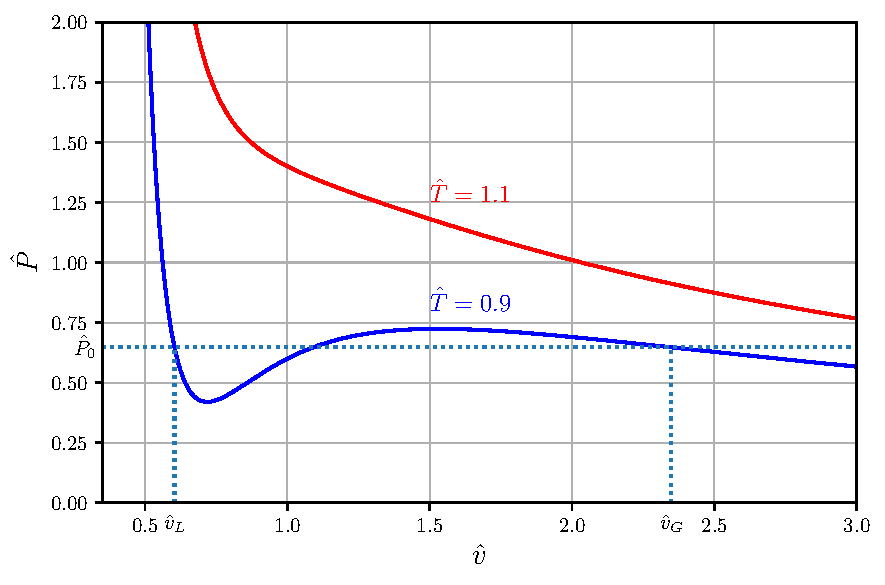
\includegraphics[width=0.6\textwidth]{figs/nle/vdw_eos.pdf}
\end{center}
% \caption{Solutions to the van der Waals equation at different temperatures. The number of real roots depends on the thermodynamic conditions.}
% \end{figure}

Depending on the values of $\hat{P}$ and $\hat{T}$, this equation can have 1 or 3 real solutions for the molar volume, corresponding to different phases of matter. In the plot above, we see that for a given reduced temperature $\hat{T} = 0.9$ (blue line) and reduced pressure $\hat{P} = \hat{P}_0$, there are three real solutions for the molar volume (only two of which are physically stable---the middle one leads to phase separation, as you will learn in 10.40). Meanwhile, for the higher reduced temperature $\hat{T} = 1.1$ (red line), there is only one real solution to $\hat v$ that will satisfy the original system of equations for any given value of $\hat{P}$. % TODO: update plot to show a specific intersection with \hat P_0
\end{exampleBox}
    
For linear systems $\mathbf{Ax=b}$, we have a clean criterion: the rank of $\mathbf{A}$ tells us exactly when solutions exist and how many there are. Nonlinear systems are different. There is no universal test that applies across all problems. Instead, the number of solutions depends on the specific structure of the system, and this global picture can shift as parameters vary (as illustrated, for example, by the van der Waals equation example above). Only in special cases do we have similar guarantees; for example, an $N$\textsuperscript{th} order polynomial has at most $N$ distinct roots. Without additional structure or assumptions, we cannot know in advance if a nonlinear system $\mathbf{f(x)=0}$ has no solutions, exactly one solution, or multiple solutions. The numerical methods/techniques we choose to solve systems of nonlinear equations must be robust to this uncertainty.

\section{The Jacobian}

Throughout this section of the course and beyond, when working with vector-valued functions, we will make extensive use of the \textbf{Jacobian matrix}. This is one way to refer to the first derivative of a vector-valued function.

\begin{definitionBox}
\textbf{Definition: Jacobian Matrix.}
For a function $\mathbf{f}: \mathbb{R}^M \rightarrow \mathbb{R}^N$, the Jacobian matrix $\mathbf{J}(\mathbf{x})$ is
{\renewcommand{\arraystretch}{1.5}
\begin{equation}
\mathbf{J}(\mathbf{x}) = \begin{bmatrix}
\frac{\partial f_1}{\partial x_1} & \frac{\partial f_1}{\partial x_2} & \cdots & \frac{\partial f_1}{\partial x_M} \\
\frac{\partial f_2}{\partial x_1} & \frac{\partial f_2}{\partial x_2} & \cdots & \frac{\partial f_2}{\partial x_M} \\
\vdots & \vdots & \ddots & \vdots \\
\frac{\partial f_N}{\partial x_1} & \frac{\partial f_N}{\partial x_2} & \cdots & \frac{\partial f_N}{\partial x_M}
\end{bmatrix} = \nabla_{\mathbf{x}}\mathbf{f}(\mathbf{x}) = \nabla\mathbf{f}(\mathbf{x}) \in \mathbb{R}^{N \times M}
\end{equation}
}
Note that in this section of the course, we typically deal with the case that $N=M$.
\end{definitionBox}
We'll prefer to use the notation $\mathbf{J}$ for the Jacobian matrix just to avoid confusion with the gradient of a scalar function. There are actually very deep connections between the Jacobian, the gradient, the Hessian, etc. If you're interested, you should take \href{https://github.com/mitmath/matrixcalc}{this IAP course on matrix calculus (18.063)}. For the purposes of 10.34, we do not need to worry about these deeper connections--we will talk about some of the connections once we introduce concepts in optimization later. However, it is important to be very familiar with the mechanics of computing the Jacobian and its structure/properties.

The Jacobian describes how the function $\mathbf{f}$ changes with respect to all its variables. More specifically, each column in the Jacobian describes the partial derivative of the vector-valued function with respect to a single input variable. It plays the same role for vector functions that the derivative plays for scalar functions. As such, we can think about it as the linear map that best approximates how $\mathbf f$ changes at a point $\mathbf x_0$: for any small increment $\Delta \mathbf x$, assuming that $\mathbf f$ is twice differentiable, we have
\begin{equation}
\label{eq:jacobian_approx}
\mathbf f(\mathbf x_0 + \Delta \mathbf x) = \mathbf f(\mathbf x_0) + \mathbf{J}(\mathbf x_0) \Delta \mathbf x  + O(\|\Delta \mathbf x\|_2^2)
\end{equation}
\autoref{eq:jacobian_approx} represents a Taylor expansion of the function $\mathbf f$ around $\mathbf x_0$, which we will elaborate on later in \autoref{sec:sne_linearization_taylor}. The higher-order terms involving the second, third, etc. derivatives of the function are omitted and replaced with the expression $O(\|\Delta \mathbf x\|_2^2)$ that defines how the truncation error scales with the magnitude of our increment $\Delta \mathbf x$. We expect the truncated linear approximation to be increasingly accurate as $\|\Delta \mathbf x\|_2 \to 0$. 

\section{Local Uniqueness}

Before we look into numerical methods to help us find solutions to nonlinear equations, we can first consider analyzing a hypothetical solution $\mathbf{x^*}$ assuming that $\mathbf{f(x^*)=0}$, i.e., that it is indeed a solution to our original system of equations. The concept of local uniqueness is an important aspect of a solution.

\begin{definitionBox}
\textbf{Definition: Local Uniqueness.}
A solution $\mathbf{x}^*$ is \textbf{locally unique} if there exists a ball of finite radius $r > 0$ such that $\mathbf{x}^*$ is the only solution within that ball:
\begin{equation}
\|\mathbf{x} - \mathbf{x}^*\| < r \quad \text{and} \quad \mathbf{f}(\mathbf{x}) = \mathbf{0} \implies \mathbf{x} = \mathbf{x}^*
\end{equation}
\end{definitionBox}  


It turns out that evaluating the Jacobian at a solution $\mathbf x^*$ allows us to easily determine local uniqueness.

\begin{theoremBox}
    \textbf{Inverse Function Theorem}
    Let $\mathbf{f}:\mathbb{R}^N \to \mathbb{R}^N$ be differentiable on an open neighborhood of $\mathbf{x}^*$, and suppose that its Jacobian $\mathbf{J}(\mathbf{x})$ varies continuously with $\mathbf{x}$ near $\mathbf{x}^*$ (i.e., $\mathbf{f}$ has a continuous derivative in a neighborhood of $\mathbf{x}^*$). If $\mathbf{f}(\mathbf{x}^*)=\mathbf{0}$ and $\det \mathbf{J}(\mathbf{x}^*)\neq 0$, then $\mathbf{x}^*$ is the unique solution of $\mathbf{f}(\mathbf{x})=\mathbf{0}$ in the neighborhood of $\mathbf{x}^*$ (i.e., the solution is locally unique).
\end{theoremBox}

This theorem generalizes the inverse function theorem from single-variable calculus to higher dimensions. There are two main ideas to highlight. First, the conditions it gives are sufficient to guarantee local uniqueness of a solution:
\begin{enumerate}
\item the function must vanish at the root, and
\item the Jacobian at that root must be nonsingular.
\end{enumerate}
Second, and equally important, we must be careful about what happens when the Jacobian is singular. A singular Jacobian does \emph{not} automatically mean the solution is not locally unique. In this case, uniqueness may or may not hold; it depends on the specific function and the particular root.

\begin{figure}[H]
\begin{center}
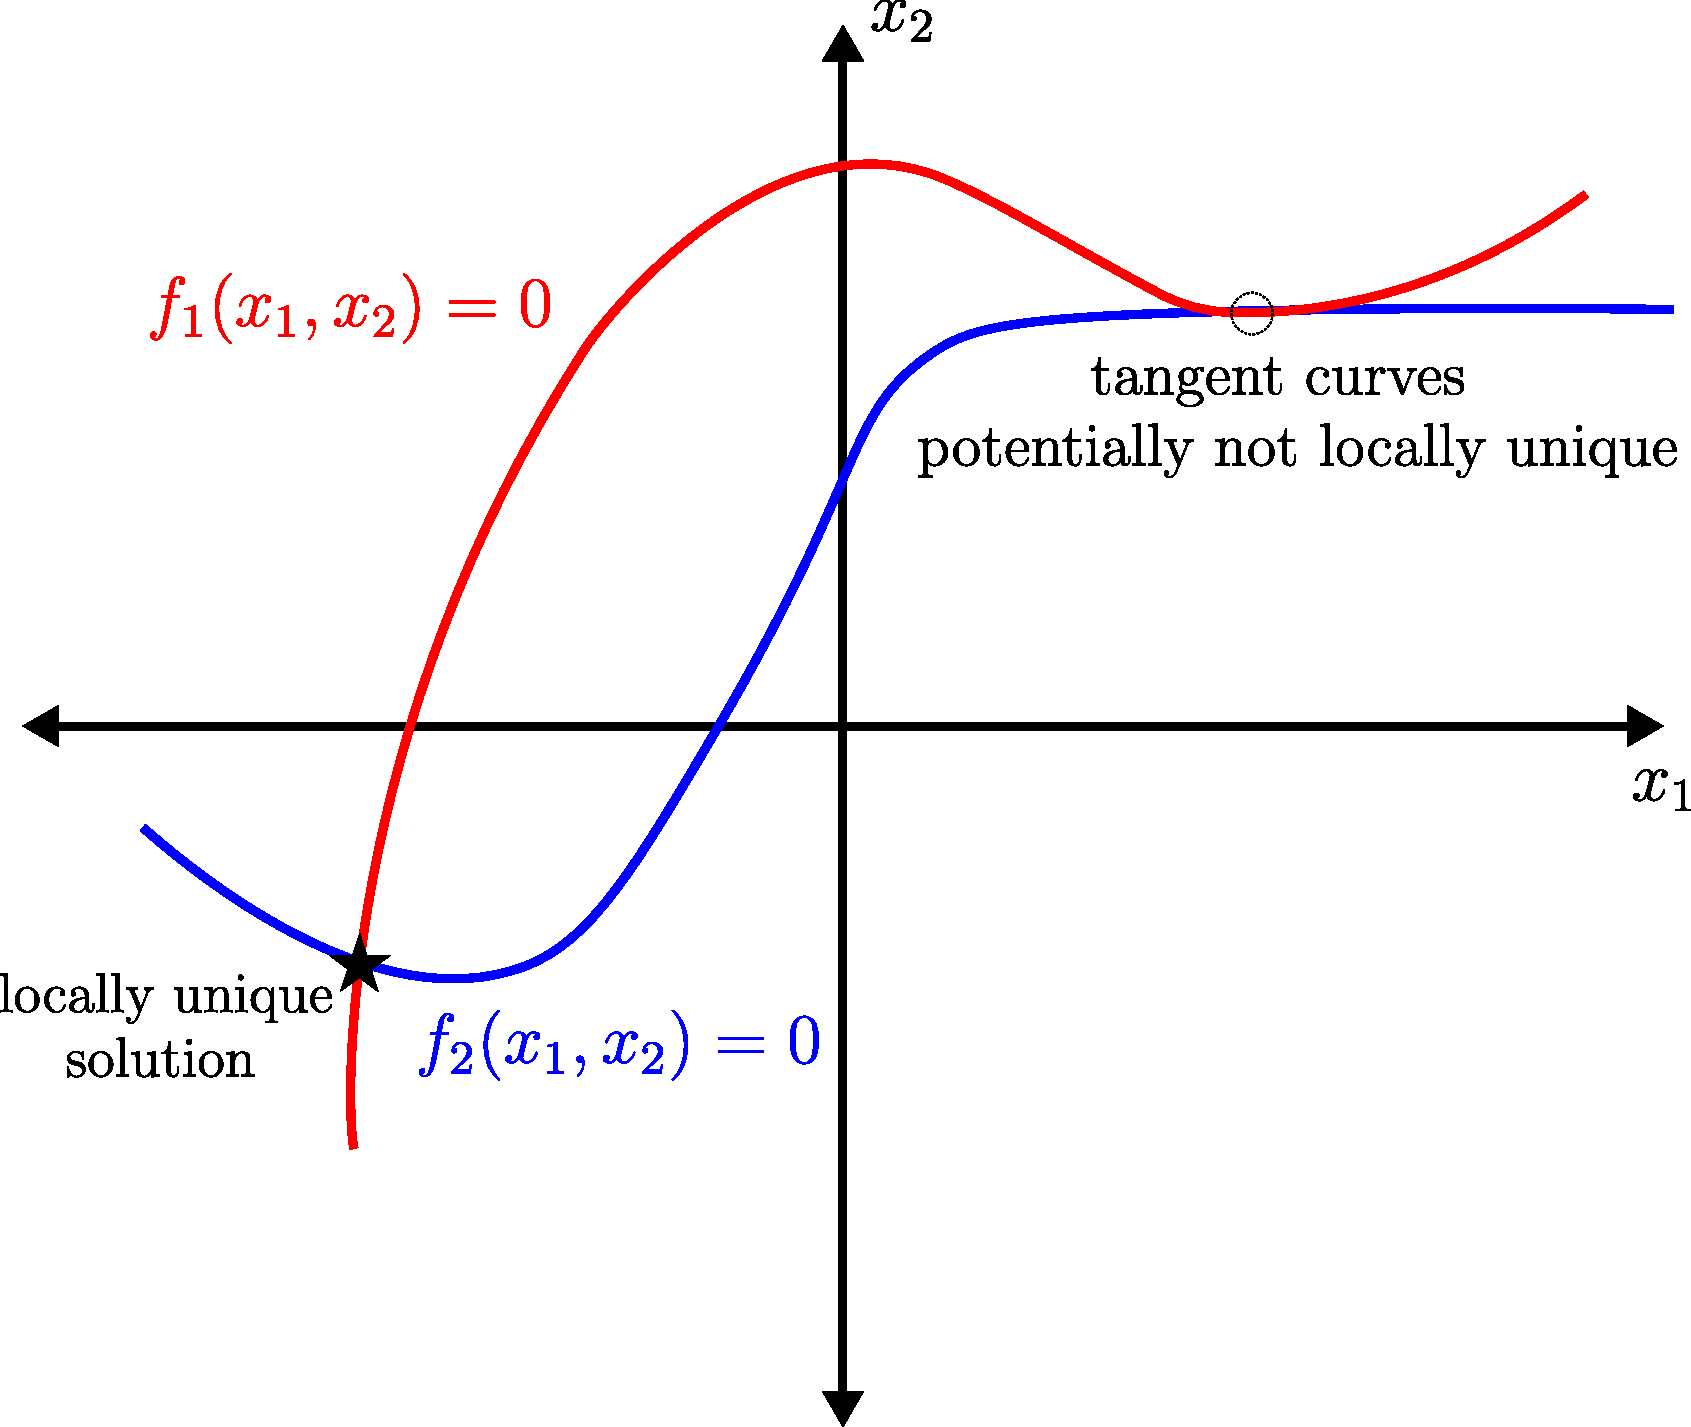
\includegraphics[width=0.6\textwidth]{figs/nle/local_uniqueness.pdf}
\caption{Application of the inverse function theorem 2D. The red and blue lines indicate the values of $x_1$ and $x_2$ for which two components of a vector-valued function, $f_1$ and $f_2$ respectively, are zero. Intersections of these curves define the roots of the function. Where the curves are tangent to each other indicates that their gradients with respect to $x_1$ and $x_2$ will be parallel, and hence the rows of the Jacobian will be linearly dependent, rendering it singular. Star: A solution where the curves intersect transversely; the Jacobian is clearly nonsingular, and therefore the solution is guaranteed to be locally unique. Dashed circle: A solution where the curves are tangent; the Jacobian is singular, and therefore the solution is \emph{potentially} non-unique. }
\end{center}
\end{figure}

A good way to see this is to compare with the single-variable setting. There, the analogous\footnote{Okay, this is not really ``analogous'' so much as it is the exact same condition. If this imprecision in language bothers you, you should definitely take 18.063 over IAP!} condition is that the derivative at the root should be nonzero. If the derivative vanishes, the situation is ambiguous: for instance, $f(x) = x^3$ has a unique root at $x=0$ even though $f'(0) = 0$, whereas $f(x) = 0$ has infinitely many roots (all $x$) and uniqueness clearly fails in a local sense at $x=0$. The multivariable case mirrors this: a nonsingular Jacobian guarantees local uniqueness, but a singular one leaves the question open.

\begin{warningBox}
    \textbf{Warning:} The converse of the inverse function theorem is not always true. In other words, we may ask, ``If $\mathbf x^*$ is a locally unique root of $\mathbf f(\mathbf x)=0$, must $\det \mathbf J(\mathbf x^*)\neq0$?'' The answer is no. Local uniqueness of the solution is strictly weaker than non-singularity of the Jacobian.  A simple one-dimensional counterexample is
    $$
      f(x) = x^3,\quad f(0)=0,\; f'(0)=0
    $$
    Here, $x=0$ is \textit{the only} solution of $f(x)=0$ in any neighborhood of 0, yet $f'(0)=0$.  So you can have a unique root even though the Jacobian vanishes at that root.
\end{warningBox}



% \begin{exampleBox}
% \textbf{Example: Computing a Jacobian}

% For the function
% \begin{equation}
% \mathbf{f}(\mathbf{x}) = \begin{bmatrix}
% x_1^2 + x_2^2 \\
% x_1^2 x_2^2
% \end{bmatrix}
% \end{equation}

% The Jacobian is
% \begin{equation}
% \mathbf{J}(\mathbf{x}) = \begin{bmatrix}
% 2x_1 & 2x_2 \\
% 2x_1x_2^2 & 2x_1^2x_2
% \end{bmatrix}
% \end{equation}

% To check local uniqueness at a root, we would evaluate $\det \mathbf{J}$ at that point.
% \end{exampleBox}

\begin{exampleBox}
    \textbf{Example: Jacobian and Uniqueness for an Exponential System}
    
    Consider the map $\mathbf{f}:\mathbb{R}^2\to\mathbb{R}^2$ given by
    \[
    \mathbf{f}(x,y)
    = \begin{bmatrix}
    x e^y - 1 \\[6pt]
    x e^{-y} - 1
    \end{bmatrix}
    \]
    Its Jacobian matrix is
    \[
    \mathbf{J}(x,y)
    = \begin{bmatrix}
    \frac{\partial}{\partial x}(x e^y - 1) & \frac{\partial}{\partial y}(x e^y - 1) \\[6pt]
    \frac{\partial}{\partial x}(x e^{-y} - 1) & \frac{\partial}{\partial y}(x e^{-y} - 1)
    \end{bmatrix}
    = \begin{bmatrix}
    e^y      & x e^y \\[4pt]
    e^{-y}   & -x e^{-y}
    \end{bmatrix}
    \]
    To find a root $\mathbf{f}(x,y)=\mathbf{0}$, we solve
    \[
    x e^y = 1,
    \quad
    x e^{-y} = 1
    \]
    Multiplying the two equations gives $x^2=1$, so $x=\pm1$.  If $x=1$, then $e^y=1$ so $y=0$.  If $x=-1$, there is no real $y$ with $e^y=-1$.  Thus, the unique real solution is
    \[
    (x,y) = (1,0)
    \]
    \textbf{Uniqueness check.}  We now verify local uniqueness at the solution by checking the determinant of the Jacobian there:
    \[
    \det \mathbf{J}(1,0)
    = \left(e^0\right)\cdot\left(-1\cdot e^0\right)
    - \left(1\cdot e^0\right)\cdot\left(e^0\right)
    = -1 - 1
    = -2 \neq 0
    \]  
    Since $\det\mathbf{J}(1,0)\neq0$, the inverse function theorem guarantees the root $(1,0)$ is locally unique.

    We can also visually verify this result from the plot of the contours of $f_1(x,y)=0$ and $f_2(x,y)=0$ below. It is obvious that the only point where the contours intersect is at $(1,0)$ and that this point is locally unique.
    \begin{center}
    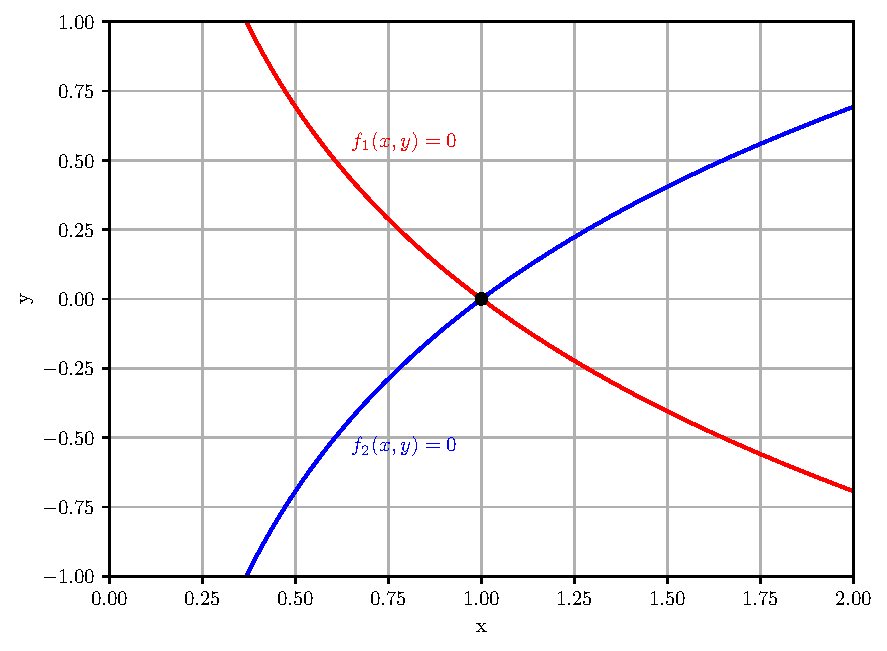
\includegraphics[width=0.6\textwidth]{figs/nle/exponential_example.pdf}
    \end{center}
\end{exampleBox}

\section{Connection to Linear Systems}

There's a deep connection between nonlinear systems and the linear systems we studied earlier. Consider a linear system $\mathbf{f}(\mathbf{x}) = \mathbf{A}\mathbf{x} - \mathbf{b}$. The Jacobian is simply
\begin{equation}
\mathbf{J}(\mathbf{x}) = \mathbf{A}
\end{equation}
(To see this, it's easiest to use the notion of the Jacobian given by \autoref{eq:jacobian_approx}. We can read off the derivative of $\mathbf f$ by looking at how $\mathbf f$ changes under a small increment, and in this case it's simply $\mathbf A$. The \href{https://www.math.uwaterloo.ca/~hwolkowi/matrixcookbook.pdf}{Matrix Cookbook} is a terrific resource for more complex identities than this.)

The condition for local uniqueness, $\det \mathbf{J}(\mathbf{x}) \neq 0$, becomes $\det \mathbf{A} \neq 0$, which is exactly the condition for $\mathbf{A}$ to be invertible! For systems of linear equations, we know that if $\mathbf{Ax=b}$ has a solution $\mathbf x^*$, that solution is guaranteed to be (locally) unique if $\mathbf{A}$ is nonsingular. So, our theory of nonlinear equations naturally extends our understanding of linear systems.

\section{Linearization via Taylor Expansions}
\label{sec:sne_linearization_taylor}
A Taylor expansion of a sufficiently smooth (this is usually a safe assumption in 10.34) vector-valued function 
\(\mathbf f\colon\mathbb R^N\to\mathbb R^N\) about the point \(\mathbf x\) shows that, for any small increment \(\Delta\mathbf x\in\mathbb R^N\),
\begin{equation}
\mathbf f(\mathbf x + \Delta\mathbf x) = \mathbf f(\mathbf x) +\mathbf{J}(\mathbf x) \Delta\mathbf x +O\bigl(\|\Delta\mathbf x\|_2^2\bigr)
\end{equation}
where the Jacobian \(\mathbf{J}(\mathbf x)\) is exactly the matrix of first-order partial derivatives defined earlier.  In one dimension, this reduces to the familiar result that
\begin{equation}
f(x+\Delta x)=f(x)+f'(x)\Delta x+ O(\Delta x^2)
\end{equation}
again making it clear that \(\mathbf{J}(\mathbf x)\) plays the role of the derivative in higher dimensions.

\subsection{Local Uniqueness via Taylor Expansions}
To see how this yields local uniqueness of a root, suppose \(\mathbf x^*\) satisfies \(\mathbf f(\mathbf x^*)= \mathbf 0\).  A Taylor expansion about \(\mathbf x^*\) gives
\begin{equation}
\mathbf f(\mathbf x)
=\cancelto{\mathbf0}{\mathbf f(\mathbf x^*)}
+\mathbf J(\mathbf x^*)\bigl(\mathbf x-\mathbf x^*\bigr)
+ O\bigl(\|\mathbf x-\mathbf x^*\|^2\bigr)
=\mathbf J(\mathbf x^*) \Delta\mathbf x
+\underbrace{O\bigl(\|\Delta\mathbf x\|^2\bigr)}_{\mathbf{R}(\Delta\mathbf x)}
\end{equation}
where \(\Delta\mathbf x=\mathbf x-\mathbf x^*\).  Here, the remainder term \(\mathbf{R}(\Delta\mathbf x) \triangleq O(\|\Delta\mathbf x\|^2)\) denotes an error that vanishes faster than \(\|\Delta\mathbf x\|\) as \(\mathbf x\to\mathbf x^*\), so for sufficiently small \(\Delta\mathbf x\) the linear part dominates.

If \(\det \mathbf J(\mathbf x^*)\neq 0\), the matrix \(\mathbf J(\mathbf x^*)\) is invertible and its null-space consists only of the zero vector.  We can prove the inverse function theorem using a proof by contradiction. Suppose that there were a distinct root \(\mathbf x=\mathbf x^*+\Delta\mathbf x\) with \(0<\|\Delta\mathbf x\|\ll1\). If this is a root, then \(\mathbf f(\mathbf x^*+\Delta\mathbf x) = \mathbf 0\) by definition. Therefore, % TODO: This mini proof can probably be simplified to match what is discussed in lecture
\begin{equation}
\mathbf{0} = \mathbf J(\mathbf x^*) \Delta\mathbf x + \mathbf{R}(\Delta\mathbf x) \implies
\mathbf J(\mathbf x^*) \Delta\mathbf x = - \mathbf{R}(\Delta\mathbf x)
\end{equation}
Since \(\mathbf J(\mathbf x^*)\) is invertible, we can solve for \(\Delta\mathbf x\):
\begin{equation}
\Delta\mathbf x = - \mathbf J(\mathbf x^*)^{-1} \mathbf{R}(\Delta\mathbf x)
\end{equation}
Now, taking norms on both sides, we have
\begin{equation}
\|\Delta\mathbf x\|
=\bigl\|\mathbf J(\mathbf x^*)^{-1}\mathbf{R}(\Delta\mathbf x)\bigr\|
\le \bigl\|\mathbf J(\mathbf x^*)^{-1}\bigr\|\bigl\|\mathbf{R}(\Delta\mathbf x)\bigr\|
\end{equation}
By the definition of $\mathbf R$, there exists $C>0$ with
$\|\mathbf R(\Delta\mathbf x)\|\le C\|\Delta\mathbf x\|^2$ for small $\|\Delta\mathbf x\|$.
Hence
\begin{equation}
\|\Delta\mathbf x\|
\le \|\mathbf J(\mathbf x^*)^{-1}\|\,C\,\|\Delta\mathbf x\|^2
\end{equation}
If $0<\|\Delta\mathbf x\|<(\|\mathbf J(\mathbf x^*)^{-1}\|\,C)^{-1}$, then dividing by $\|\Delta\mathbf x\|$ yields $1\le \|\mathbf J(\mathbf x^*)^{-1}\|\,C\,\|\Delta\mathbf x\|<1$, a contradiction. Therefore, $\Delta\mathbf x=0$ is the only possibility in a sufficiently small neighborhood, which completes the argument that no other root can lie nearby.

\begin{exampleBox}
\textbf{Example: Visualizing the Quadratic Remainder}
Consider the scalar (1D) function
\[
f(x) = x + x^3
\]
which has a simple root at \(x^*=0\).  We plot \(f(x)\) together with its tangent line (first-order Taylor approximation)
\(\ell(x)=f'(x^*)(x-x^*)\), and we shade the region where the Taylor remainder satisfies
\(\lvert R(\Delta x)\rvert \le C \cdot (\Delta x)^2\).  Concretely, we choose a small radius \(r\) and display
the band \(\pm(\Delta x)^2\) for \(\lvert x-x^*\rvert\le r\).  Since the tangent line crosses the axis
only once and the nonlinear curve stays inside this narrow tube, no second root can lie in that
neighborhood, visually confirming the local uniqueness result.

\begin{center}
    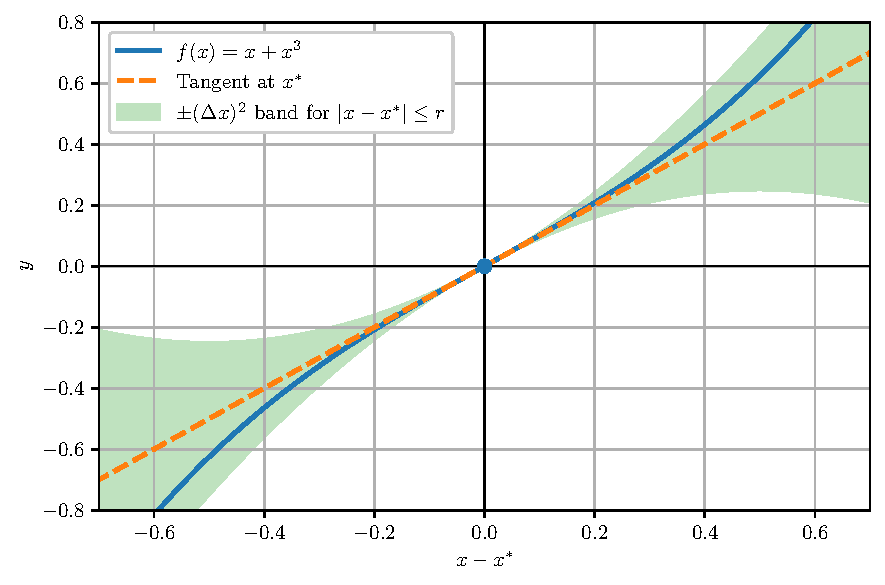
\includegraphics[width=0.6\textwidth]{figs/nle/tangent_band.pdf}
\end{center}
% \caption{%
%   A scalar function $f(x)=x+x^3$ (solid), its tangent line at the simple root $x^*=0$ (dashed), 
%   and the quadratic error band $\pm x^2$ for $|x-x^*|\le r$ (shaded).}
% \label{fig:tangent-band}
\end{exampleBox}

\section{Iterative Methods for Solving Nonlinear Equations}

We are concerned with finding solutions $\vect{x}^* \in \mathbb{R}^N$ to a system of $n$ nonlinear equations $\vect{f}(\vect{x}) = \vect{0}$, where $\vect{f}: \mathbb{R}^N \to \mathbb{R}^N$:
\begin{equation}
    \vect{f}(\vect{x}^*) = \begin{bmatrix} f_1(x_1^*, x_2^*, \dots, x_N^*) \\ f_2(x_1^*, x_2^*, \dots, x_N^*) \\ \vdots \\ f_N(x_1^*, x_2^*, \dots, x_N^*) \end{bmatrix} = \begin{bmatrix} 0 \\ 0 \\ \vdots \\ 0 \end{bmatrix} = \vect{0}
\end{equation}
Unlike linear systems, most nonlinear systems do not admit a closed-form solution. Therefore, we almost always resort to iterative methods. An iterative method generates a sequence of approximate solutions $\{\vect{x}_k\}$ starting from an initial guess $\vect{x}_0$ with the aim that this sequence converges to a true solution $\vect{x}^*$, i.e., $\lim_{k\to\infty} \vect{x}_k = \vect{x}^*$. 

Many iterative methods make use of  \textbf{fixed-point iteration}. The idea is to transform the original root-finding problem $\vect{f}(\vect{x}) = \vect{0}$ into an equivalent fixed-point problem of the form
\begin{equation}
    \vect{x} = \vect{g}(\vect{x})
    \label{eq:fixed_point_iteration}
\end{equation}
$\vect{g}$ serves as a map from any provided value of $\mathbf x$ to an updated value. Given an initial value $\mathbf x_0$, we feed it into the function to get $\mathbf x_1 = \mathbf g(\mathbf x_0)$, then again to get $\mathbf x_2 = \mathbf g(\mathbf x_1)$, and so on.

Depending on the definition of $\mathbf g$, there may be special values of $\mathbf x$ that remain unchanged by $\mathbf g$ and, therefore, correspond to solutions to the fixed-point problem \autoref{eq:fixed_point_iteration}. More formally, a solution $\vect{x}^*$ to this equation is called a fixed point of the function $\vect{g}$ if applying $\vect{g}$ to $\vect{x}^*$ yields $\vect{x}^*$ itself: $\vect{x}^* = \vect{g}(\vect{x}^*)$. 

The key idea is to construct $\vect{g}(\vect{x})$ such that any fixed point of $\vect{g}$ is also a root of $\vect{f}$. When we can ensure this is the case, identifying solutions to $\mathbf f(\mathbf x) = \mathbf 0$ becomes equivalent to finding these fixed points. There are many ways to define such a $\vect{g}(\vect{x})$. A common family of transformations is
\begin{equation}
    \vect{g}(\vect{x}) = \vect{x} + \mat{A}(\vect{x})\vect{f}(\vect{x})
\end{equation}
where $\mat{A}(\vect{x})$ is a suitably chosen matrix (which could be constant, or depend on $\vect{x}$ as suggested by the notation). If $\vect{x}^* = \vect{g}(\vect{x}^*)$, then $\vect{x}^* = \vect{x}^* + \mat{A}(\vect{x}^*)\vect{f}(\vect{x}^*)$, which implies $\mat{A}(\vect{x}^*)\vect{f}(\vect{x}^*) = \vect{0}$. If $\mat{A}(\vect{x}^*)$ is non-singular, then this ensures $\vect{f}(\vect{x}^*) = \vect{0}$. Once the problem is in fixed-point form, the iteration proceeds as
\begin{equation}
    \vect{x}_{k+1} = \vect{g}(\vect{x}_k), \quad k = 0, 1, 2, \dots
\end{equation}
If this sequence converges, i.e., $\vect{x}_k \to \vect{x}^*$ as $k \to \infty$, and if $\vect{g}$ is continuous in a neighborhood of $\vect{x}^*$, then taking the limit on both sides gives
\begin{equation} 
\lim_{k\to\infty} \vect{x}_{k+1} = \lim_{k\to\infty} \vect{g}(\vect{x}_k) \implies \vect{x}^* = \vect{g}(\vect{x}^*) 
\end{equation}
Thus, the limit, if it exists, is indeed a fixed point of $\vect{g}$ and, by construction, a solution to $\vect{f}(\vect{x}) = \vect{0}$.

\subsection{Stopping Criteria}
In practice, iterative methods cannot run indefinitely. We need criteria to decide when an iterate $\vect{x}_k$ is ``close enough'' to the true solution $\vect{x}^*$ to stop the process. Since $\vect{x}^*$ is generally unknown, these criteria are based on observable quantities. Two common stopping criteria are as follows:

\begin{enumerate}
    \item \textbf{Function Norm (Residual) Test}\footnote{We call this a residual test because in this case, the residual is by definition $\vect{R}_{k+1} = \vect{f}(\vect{x}_{k+1}) - \vect{0} = \vect{f}(\vect{x}_{k+1})$}: This criterion checks if the function value $\vect{f}(\vect{x}_{k+1})$ is close to zero.
    \begin{equation}
        \|\vect{f}(\vect{x}_{k+1})\|_p \le \varepsilon_f
    \end{equation}
    Here, $\|\cdot\|_p$ denotes a chosen vector $p$-norm (e.g., $p=1, 2, \infty$), and $\varepsilon_f > 0$ is a prescribed absolute tolerance for the residual. A small residual means that $\vect{x}_{k+1}$ nearly satisfies the system of equations.

    \item \textbf{Step Size (Iterate Difference) Test}: This criterion checks if the change between successive iterates is small.
    \begin{equation}
        \|\vect{x}_{k+1} - \vect{x}_k\|_p \le \varepsilon_R \|\vect{x}_{k+1}\|_p + \varepsilon_A
    \end{equation}
    Here, $\varepsilon_R \ge 0$ is a relative tolerance and $\varepsilon_A \ge 0$ is an absolute tolerance. This test helps detect when the iteration is no longer making significant progress. The relative tolerance $\varepsilon_R \|\vect{x}_{k+1}\|_p$ is useful when the magnitude of $\vect{x}_{k+1}$ is large, while the absolute tolerance $\varepsilon_A$ is important when $\vect{x}_{k+1}$ is close to zero.
\end{enumerate}
Often, a combination of these tests (or others, like a maximum iteration count or detection of NaNs/infs) is used.

\subsubsection{Failure Modes of Stopping Criteria}
While standard, these stopping criteria are far from foolproof and can sometimes indicate convergence prematurely or fail to indicate convergence when it occurs slowly.

\textbf{Residual Test Failure:}
A small residual $\|\vect{f}(\vect{x}_k)\|$ does not always imply that $\vect{x}_k$ is close to $\vect{x}^*$. If the function $\vect{f}$ is very ``flat'' near the root (i.e., its Jacobian is ill-conditioned or nearly singular), then many points $\vect{x}$ far from $\vect{x}^*$ can have small function values. Geometrically, $\vect{x}_k$ might be on a nearly level set of $\vect{f}$ close to zero, but this level set could be wide.

\begin{figure}[h]
    \centering
    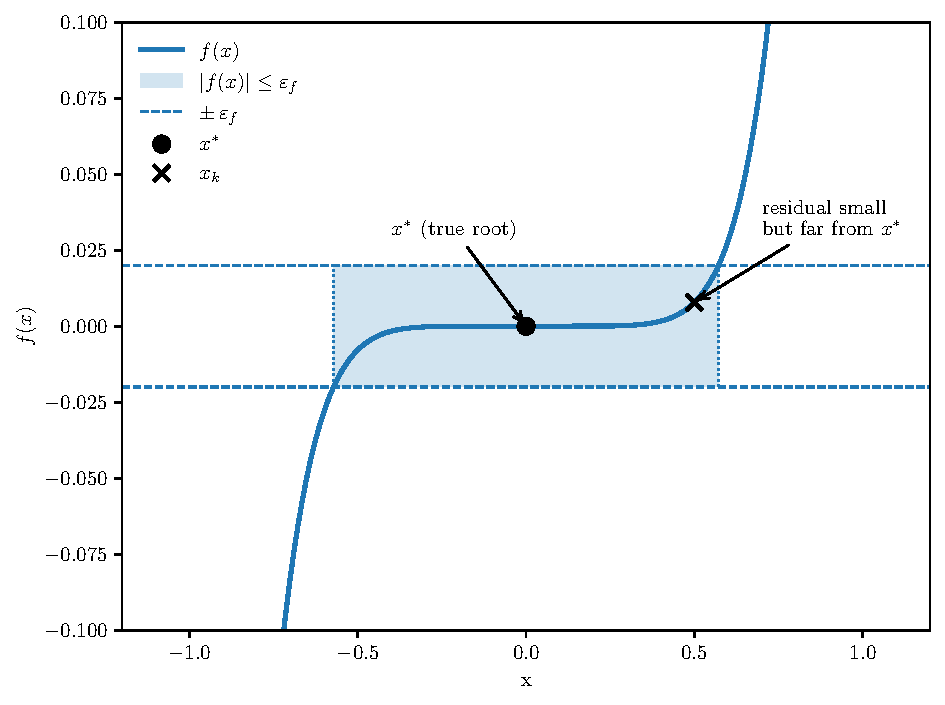
\includegraphics[width=0.5\textwidth]{figs/nle/residual_test_failure.pdf}
    \caption{Failure of the residual test: A small residual $\|\vect{f}(\vect{x}_k)\| \le \varepsilon_f$ may occur even if $\vect{x}_k$ is far from the true root $\vect{x}^*$, especially if $\vect{f}$ is flat near $\vect{x}^*$.}
\end{figure}


\textbf{Step-Size Test Failure:}
A small step size $\|\vect{x}_{k+1} - \vect{x}_k\|$ only means that the iteration has stalled or is converging very slowly. The iterates might be making negligible progress while still being far from any actual root, or they could be slowly converging in a narrow valley region of the function landscape.

\begin{figure}[H]
    \centering
    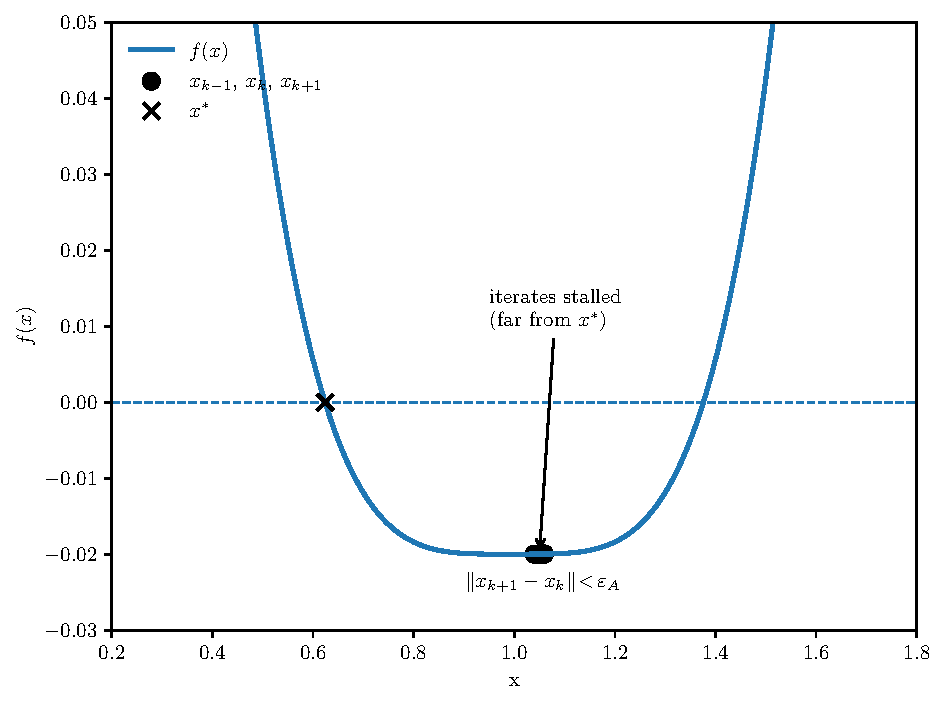
\includegraphics[width=0.5\textwidth]{figs/nle/stepsize_test_failure.pdf}
    \caption{Failure of the step-size test: Successive iterates $\vect{x}_k$ and $\vect{x}_{k+1}$ may be very close, indicating stalled progress, even if they are far from the true root $\vect{x}^*$.}
\end{figure}

It is generally advisable to use a combination of these criteria and to have some understanding of the problem's characteristics.

\subsection{Convergence Analysis}
The speed at which an iterative method $\vect{x}_{k+1} = \vect{g}(\vect{x}_k)$ converges to a root $\vect{x}^*$ is an important characteristic. Let $\vect{e}_k = \vect{x}_k - \vect{x}^*$ be the error at iteration $k$. The iteration is said to converge with order $q \ge 1$ if there exists a constant $C$ (called the asymptotic error constant) with $0<C<\infty$ such that
\begin{equation}
    \lim_{k\to\infty} \frac{\|\vect{e}_{k+1}\|_p}{\|\vect{e}_k\|_p^{\,q}} = C
\end{equation}
We can take a look at some common convergence orders. \textbf{Linear convergence} occurs if $q=1$ and $0<C<1$. The error is reduced by a roughly constant factor at each step. The number of correct significant digits increases linearly with $k$; more precisely, digits gained per step $\approx -\log_{10} C$. For example, if $C \approx 0.1$, about one new correct digit is gained per iteration. Classical stationary methods like Jacobi and Gauss-Seidel for linear systems exhibit linear convergence under standard assumptions (e.g., when the iteration matrix has spectral radius $<1$).

\textbf{Superlinear convergence} occurs if $q>1$. Equivalently, we can characterize it by
\begin{equation}
  \lim_{k\to\infty}\frac{\|\vect{e}_{k+1}\|_p}{\|\vect{e}_k\|_p}=0
\end{equation}
which corresponds informally to the $q=1$ case with $C=0$ (noting this lies outside the $0<C<\infty$ definition above). This is faster than linear.

\textbf{Quadratic convergence} occurs if $q=2$. The number of correct significant digits roughly doubles at each iteration, leading to very rapid convergence once the iterates are close to the root.

In finite dimensions, the choice of $p$-norm does not affect the order $q$ (all norms are equivalent), though the constant $C$ may change.



\subsection{The Newton-Raphson Method}
The Newton-Raphson method, often just called Newton's method, is one of the most powerful and widely used iterative algorithms for finding roots of nonlinear equations. Its strength lies in its typically fast convergence rate when the initial guess is sufficiently close to the root.

Newton's method can be viewed as a specific instance of fixed-point iteration. As we will see, the iteration function $\vect{g}(\vect{x})$ is chosen based on a linear approximation of $\vect{f}(\vect{x})$ at the current iterate. Specifically, if we consider the general fixed-point construction $\vect{g}(\vect{x}) = \vect{x} + \mat{A}(\vect{x})\vect{f}(\vect{x})$, Newton's method makes the choice $\mat{A}(\vect{x}_k) = -[\mat{J}(\vect{x}_k)]^{-1}$, where $\mat{J}(\vect{x}_k)$ is the Jacobian matrix of $\vect{f}$ evaluated at $\vect{x}_k$. This leads to the iteration:
\begin{equation}
    \vect{x}_{k+1} = \vect{x}_k - [\mat{J}(\vect{x}_k)]^{-1} \vect{f}(\vect{x}_k)
\end{equation}
We can understand where this comes from quite easily by considering a first-order Taylor expansion of $\vect{f}(\vect{x})$ around the current iterate $\vect{x}_k$. For an increment $\Delta\vect{x} = \vect{x} - \vect{x}_k$, we have the expansion
\begin{equation}
    \vect{f}(\vect{x}_k + \Delta\vect{x}) \approx \vect{f}(\vect{x}_k) + \mat{J}(\vect{x}_k) \Delta\vect{x}
\end{equation}
where $\mat{J}(\vect{x}_k)$ is the Jacobian matrix (with elements $J_{ij}(\vect{x}_k) = \tfrac{\partial f_i}{\partial x_j}(\vect{x}_k)$ as always). Newton's method tries to find the next iterate $\vect{x}_{k+1}$ such that the linear model predicts $\vect{f}(\vect{x}_{k+1}) = \vect{0}$. Let $\vect{x}_{k+1} = \vect{x}_k + \vect{d}_k$, where $\vect{d}_k$ is the step/correction/displacement. Substituting this into the linearized equation, we get
\begin{equation}
    \vect{0} \approx \vect{f}(\vect{x}_k) + \mat{J}(\vect{x}_k) \vect{d}_k
\end{equation}
This can be rearranged into a system of linear equations for the unknown step $\vect{d}_k$:
\begin{equation}
    \mat{J}(\vect{x}_k) \vect{d}_k = -\vect{f}(\vect{x}_k)
\end{equation}
Assuming the Jacobian $\mat{J}(\vect{x}_k)$ is non-singular, we can solve for $\vect{d}_k$:
\begin{equation}
    \vect{d}_k = -[\mat{J}(\vect{x}_k)]^{-1} \vect{f}(\vect{x}_k)
\end{equation}
The next iterate is then found by updating the current one:
\begin{equation}
    \vect{x}_{k+1} = \vect{x}_k + \vect{d}_k = \vect{x}_k - [\mat{J}(\vect{x}_k)]^{-1} \vect{f}(\vect{x}_k)
\end{equation}
Each step of Newton's method thus involves:
\begin{enumerate}
    \item Evaluating the function $\vect{f}(\vect{x}_k)$ and the Jacobian matrix $\mat{J}(\vect{x}_k)$ at the current iterate $\vect{x}_k$.
    \item Solving the linear system $\mat{J}(\vect{x}_k)\vect{d}_k = -\vect{f}(\vect{x}_k)$ for the step $\vect{d}_k$.
    \item Updating the iterate: $\vect{x}_{k+1} = \vect{x}_k + \vect{d}_k$.
\end{enumerate}
We very rarely compute the inverse $[\mat{J}(\vect{x}_k)]^{-1}$ explicitly. Instead, the linear system for $\vect{d}_k$ is solved numerically (using, for example, the techniques discussed earlier) for better efficiency.

\textbf{Scalar Case (1D Newton's Method):}
For a single scalar function $f(x)$ (where $f:\mathbb{R}\to\mathbb{R}$), the derivation simplifies considerably. The Jacobian matrix $\mat{J}(x_k)$ becomes the scalar first derivative $f'(x_k)$. The Taylor expansion is
\begin{equation}
    f(x) \approx f(x_k) + f'(x_k)(x - x_k)
\end{equation}
We want to find $x_{k+1}$ such that this linear approximation is zero:
\begin{equation}
    0 = f(x_k) + f'(x_k)(x_{k+1} - x_k)
\end{equation}
Solving for $x_{k+1}$, assuming $f'(x_k) \neq 0$,
\begin{equation}
    f'(x_k)(x_{k+1} - x_k) = -f(x_k)
\end{equation}
\begin{equation}
    x_{k+1} - x_k = -\frac{f(x_k)}{f'(x_k)}
\end{equation}
\begin{equation}
    x_{k+1} = x_k - \frac{f(x_k)}{f'(x_k)}
\end{equation}
This should be quite familiar from previous calculus courses. Geometrically, $x_{k+1}$ is the point where the tangent line to the graph of $f(x)$ at $x_k$ intersects the x-axis (\autoref{fig:newton_1d}).

\begin{figure}[H]
    \centering
    \begin{tikzpicture}[>=latex, font=\small]

        % --- function and derivative (convex increasing) ---
        \def\a{0.08}            % f(x) = a x^2 + b
        \def\b{-1.2}
        \pgfmathdeclarefunction{f}{1}{\pgfmathparse{\a*#1*#1+\b}}
        \pgfmathdeclarefunction{df}{1}{\pgfmathparse{2*\a*#1}}
        
        % --- choose starting point x_n and compute Newton steps ---
        \pgfmathsetmacro{\xn}{8}
        \pgfmathsetmacro{\yn}{f(\xn)}
        \pgfmathsetmacro{\mA}{df(\xn)}
        \pgfmathsetmacro{\xnp}{\xn-\yn/\mA}
        \pgfmathsetmacro{\ynp}{f(\xnp)}
        \pgfmathsetmacro{\mB}{df(\xnp)}
        \pgfmathsetmacro{\xnpp}{\xnp-\ynp/\mB}
        \pgfmathsetmacro{\ynpp}{f(\xnpp)}
        \pgfmathsetmacro{\angA}{atan(\mA)}
        \pgfmathsetmacro{\angB}{atan(\mB)}
        
        % --- axes ---
        \draw[->] (-1,0) -- (10.5,0) node[below right] {$x$};
        \draw[->] (0,-1.5) -- (0,6.2) node[left] {$f(x)$};
        
        % --- function curve ---
        \draw[very thick]
          plot[samples=200,domain=0:9] (\x,{f(\x)}) node[pos=0.98,above] {$f(x)$};
        
        % --- tangent at x_n: y = f(x_n)+f'(x_n)(x-x_n) ---
        \draw[dashed, blue]
          plot[domain=\xnpp-0.7:\xn+1, samples=2]
            (\x,{\yn+\mA*(\x-\xn)});
        % \node[rotate=\angA, anchor=west] at (\xn+0.6,{\yn+\mA*0.6}) {$f'(x_n)$};
        
        % --- tangent at x_{n+1} ---
        \draw[dashed, red]
          plot[domain=\xnpp-0.7:\xnp+1, samples=2]
            (\x,{\ynp+\mB*(\x-\xnp)});
        % \node[rotate=\angB, anchor=west] at (\xnp+0.6,{\ynp+\mB*0.6}) {$f'(x_{n+1})$};
        
        % --- vertical guides ---
        \draw[densely dotted] (\xn,0) -- (\xn,\yn);
        \draw[densely dotted] (\xnp,0) -- (\xnp,\ynp);
        \draw[densely dotted] (\xnpp,0) -- (\xnpp,\ynpp);
        
        % --- points on the curve ---
        \fill (\xn,\yn)       circle (2pt) node[above left] {$f(x_n)$};
        \fill (\xnp,\ynp)     circle (2pt) node[above left] {$f(x_{n+1})$};
        \fill (\xnpp,\ynpp)   circle (2pt) node[above left] {$f(x_{n+2})$};
        
        % --- ticks and x-labels ---
        \draw (\xn,0.1)   -- (\xn,-0.1)   node[below] {$x_n$};
        \draw (\xnp,0.1)  -- (\xnp,-0.1)  node[below] {$x_{n+1}$};
        \draw (\xnpp,0.1) -- (\xnpp,-0.1) node[below] {$x_{n+2}$};
        
    \end{tikzpicture}
    \caption{Visual depiction of Newton's method for a scalar function $f(x)$.}
    \label{fig:newton_1d}
\end{figure}

The Newton-Raphson algorithm for systems is summarized below using both the discussed stopping criteria simultaneously.

\begin{algorithm}[H]
    \caption{Newton's Method for Systems (robust variant)}
    \begin{algorithmic}[1]
    \State Choose $\mathbf{x}_0$, tolerances $\varepsilon_f,\ \varepsilon_R,\ \varepsilon_A$, and $K_{\max}$.
    \For{$k=0,1,2,\dots,K_{\max}-1$}
        \State $\mathbf{f}_k \gets \mathbf{f}(\mathbf{x}_k)$
        \If{$\|\mathbf{f}_k\|_p \le \varepsilon_f$}
            \State \Return $\mathbf{x}_k$ \Comment{converged by residual}
        \EndIf
        \State $\mathbf{J}_k \gets \mathbf{J}(\mathbf{x}_k)$
        \State Solve $\mathbf{J}_k \mathbf{d}_k = -\mathbf{f}_k$ for $\mathbf{d}_k$ (numerically)
        \State $\mathbf{x}_{k+1} \gets \mathbf{x}_k + \mathbf{d}_k$
        \If{$\|\mathbf{d}_k\|_p \le \varepsilon_R \|\mathbf{x}_{k+1}\|_p + \varepsilon_A$}
            \State \Return $\mathbf{x}_{k+1}$ \Comment{converged by step size}
        \EndIf
    \EndFor
    \State \Return $\mathbf{x}_{k+1}$ \Comment{or best of $\mathbf{x}_k,\mathbf{x}_{k+1}$ if available}
    \end{algorithmic}
\end{algorithm}

\begin{exampleBox}
\textbf{Example: Intersection of Two Circles.}
Consider the problem of finding the intersection points of two circles:
\begin{align*}
    f_1(x_1, x_2) &= (x_1 - 2)^2 + (x_2 - 2)^2 - 9 = 0 \\
    f_2(x_1, x_2) &= (x_1 + 3)^2 + (x_2 + 1)^2 - 9 = 0
\end{align*}
Here, $\vect{x} = (x_1, x_2)^T$. The system is $\vect{f}(\vect{x}) = (f_1(\vect{x}), f_2(\vect{x}))^T = \vect{0}$.

\begin{center}
    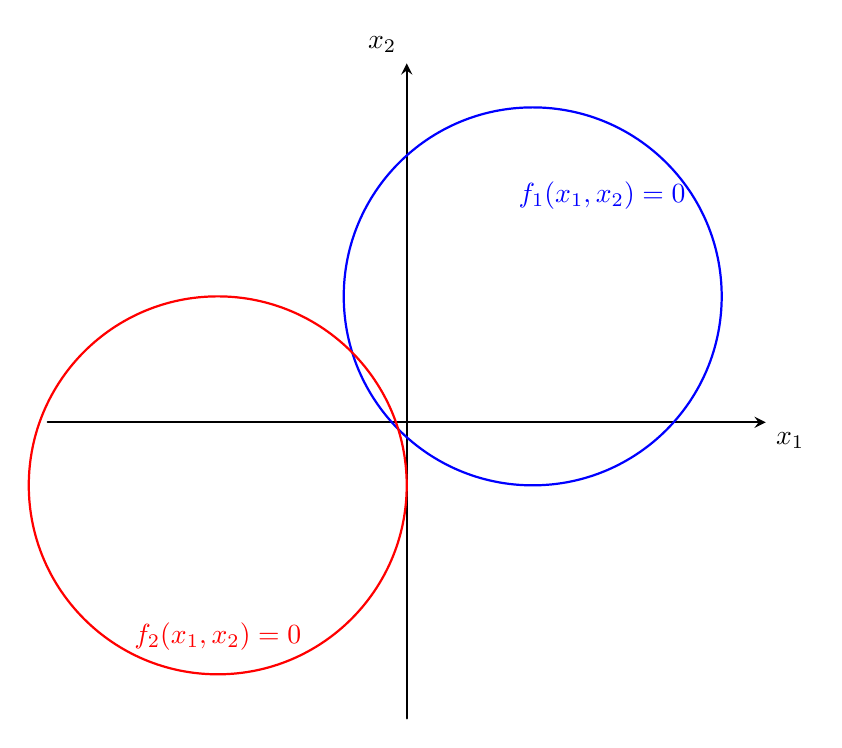
\begin{tikzpicture}[scale=0.8,>=stealth,line cap=round,line join=round]
        % Axes
        \draw[thick,->] (-5.7,0) -- (5.7,0) node[below right] {$x_1$};
        \draw[thick,->] (0,-4.7) -- (0,5.7) node[above left] {$x_2$};
      
        % Circles
        % f1(x1,x2)=0 : (x1-2)^2 + (x2-2)^2 = 3^2
        \draw[blue,thick] (2,2) circle (3);
      
        % f2(x1,x2)=0 : (x1+3)^2 + (x2+1)^2 = 3^2
        \draw[red,thick] (-3,-1) circle (3);
      
        % Labels
        \node[blue] at (3.1,3.6) {$f_1(x_1,x_2)=0$};
        \node[red]  at (-3.0,-3.4) {$f_2(x_1,x_2)=0$};
    \end{tikzpicture}
\end{center}

The Jacobian matrix $\mat{J}(\vect{x})$ is given by:
{\renewcommand*{\arraystretch}{1.5}
\[
    \mat{J}(\vect{x}) = \begin{bmatrix}
    \frac{\partial f_1}{\partial x_1} & \frac{\partial f_1}{\partial x_2} \\
    \frac{\partial f_2}{\partial x_1} & \frac{\partial f_2}{\partial x_2}
    \end{bmatrix}
    = \begin{bmatrix}
    2(x_1 - 2) & 2(x_2 - 2) \\
    2(x_1 + 3) & 2(x_2 + 1)
    \end{bmatrix}
\]
}

Starting with an initial guess, say $\vect{x}_0 = (-1, 3)^\top$, we can apply Newton's method. The table below shows the first few iterations:

\begin{center}
\begin{tabular}{@{}ccccc@{}}
\toprule
$k$ & $\vect{x}^{(k)^\top}$ & $\vect{f}(\vect{x}^{(k)})^\top$ & $\|\vect{x}^{(k)}-\vect{x}^{(k-1)}\|_2$ & $\|\vect{f}(\vect{x}^{(k)})\|_2$ \\ \midrule
0 & $(-1.000, 3.000)$ & $(1.00, 11.00)$ & --- & $11.100$ \\
1 & $(-1.250, 1.750)$ & $(1.625, 1.625)$ & $0.556$ & $2.300$ \\
2 & $(-0.963, 1.270)$ & $(0.310, 0.310)$ & $0.173$ & $0.439$ \\
3 & $(-0.875, 1.124)$ & $(0.030, 0.030)$ & $0.020$ & $0.042$ \\
4 & $(-0.864, 1.101)$ & $(0.004, 0.004)$ & $0.003$ & $0.006$ \\
\bottomrule
\end{tabular}
\end{center}

The iteration rapidly converges to one of the intersection points, approximately $(-0.864, 1.101)$. The choice of initial guess determines which of the two intersection points is found.

\end{exampleBox}

\subsection{Convergence of Newton's Method}
One of the primary reasons for Newton's method's popularity is its typically \textbf{quadratic convergence rate}, provided certain conditions are met.

% MC: I'm sorry this diverges from the slides a bit, this is the proof I had in my notes
% i found it clearer than the slides at the time I was a student
\textbf{1D Proof of Quadratic Convergence:}
Let's analyze the convergence for the scalar case 
\begin{equation}
x_{k+1} = x_k - \frac{f(x_k)}{f'(x_k)}
\end{equation}
 assuming $f'(x^*) \neq 0$. The error at iteration $k+1$ is $e_{k+1} = x_{k+1} - x^*$. This means that
\begin{equation}
    e_{k+1} = x_k - \frac{f(x_k)}{f'(x_k)} - x^* = (x_k - x^*) - \frac{f(x_k)}{f'(x_k)} = e_k - \frac{f(x_k)}{f'(x_k)}
    = \frac{e_k f'(x_k) - f(x_k)}{f'(x_k)}
\end{equation}
Now, we consider the Taylor expansion of $f(x^*)$ around $x_k$:
\begin{equation}
    f(x^*) = 0 = f(x_k) + f'(x_k)(x^* - x_k) + \frac{1}{2}f''(\xi_k)(x^* - x_k)^2
\end{equation}
for some $\xi_k$ between $x_k$ and $x^*$ (this is coming from the Lagrange-remainder form of Taylor's theorem). Rearranging this and noting $x^* - x_k = -e_k$, we get
\begin{equation}
    -f(x_k) = f'(x_k)(-e_k) + \frac{1}{2}f''(\xi_k)(-e_k)^2
    \implies
    e_k f'(x_k) - f(x_k) = \frac{1}{2}f''(\xi_k)e_k^2
\end{equation}
Substituting this back into the expression for $e_{k+1}$, we get
\begin{equation}
    e_{k+1} = \frac{\frac{1}{2}f''(\xi_k)e_k^2}{f'(x_k)} = \frac{f''(\xi_k)}{2f'(x_k)} e_k^2
    \implies
    |e_{k+1}| = \left| \frac{f''(\xi_k)}{2f'(x_k)} \right| |e_k|^2
\end{equation}
As $x_k \to x^*$, $\xi_k \to x^*$. Thus, if $f'(x^*) \neq 0$,
\begin{equation}
    \lim_{k\to\infty} \frac{|e_{k+1}|}{|e_k|^2} = \left| \frac{f''(x^*)}{2f'(x^*)} \right|
\end{equation}
So we have quadratic convergence for the 1D case provided that $f$ is twice continuously differentiable in a neighborhood of $x^*$, $f'(x^*) \neq 0$, and $x_0$ is sufficiently close to $x^*$.

\textbf{General Case (Multivariate):}
For systems of equations, Newton's method converges quadratically to $\vect{x}^*$ if:
\begin{enumerate}
    \item $\vect{x}_0$ is sufficiently close to $\vect{x}^*$.
    \item The Jacobian $\mat{J}(\vect{x}^*)$ is non-singular.
    \item The components of $\vect{f}$ are twice continuously differentiable in a neighborhood of $\vect{x}^*$.
\end{enumerate}
If $\mat{J}(\vect{x}^*)$ is singular, convergence typically degrades to at most linear or the method can fail. We omit the proof of these facts here; you don't need to know how to prove this for 10.34.

\subsubsection{Local Convergence}
The guarantee of quadratic convergence for Newton's method is \textit{local}, meaning it only holds if the initial guess $\vect{x}_0$ is ``sufficiently close'' to the actual root $\vect{x}^*$. The set of starting points from which Newton's method converges to a particular root is called the \textit{basin of attraction} (discussed more in \Cref{par:basins-of-attraction}) for that root. Good initial guesses are therefore essential for the success and efficiency of Newton's method. If the initial guess is poor, the sequence of iterates can behave erratically, diverge, or converge to an unintended root.


\subsubsection{Failure Modes of Newton's Method}
Newton's method can fail or perform poorly under certain conditions:
\begin{itemize}
    \item \textbf{Singular or Ill-conditioned Jacobian:} If $f'(x_k) \approx 0$ (in 1D) or $\mat{J}(\vect{x}_k)$ is singular or nearly singular, the step $\vect{d}_k$ can become excessively large, potentially causing the next iterate to overshoot the root wildly, or the linear system for $\vect{d}_k$ may not have a unique solution. This often occurs near local minima/maxima of $f(x)$ or in regions where components of $\vect{f}$ are insensitive to changes in some variables. This is the same failure mode as depicted in \autoref{fig:failure-modes}(a). In practice, damping/line-search or a trust-region variant (or using a pseudo-inverse when $\mat{J}(\vect{x}_k)$ is rank-deficient) mitigates these failures.

    \item \textbf{Cycling:} Iterates may enter a cycle, repeating a sequence of values without converging. For example, let $f(x)=x^3-2x+2$, so $f'(x)=3x^2-2$ and
    \[
    x_{k+1} = x_k-\frac{f(x_k)}{f'(x_k)} = x_k-\frac{x_k^3-2x_k+2}{3x_k^2-2}
    \]
    Starting at $x_0=0$,
    \[
    x_1=1,\qquad x_2 = 0 = x_0
    \]
    so the iterates enter the cycle of $0 \leftrightarrow 1$ and never converge to a root.
    
    \item \textbf{Divergence to Infinity:} Iterates may move progressively further from any root. For example, take $f(x)=\arctan x$ (root at $x^*=0$). Then $f'(x)=1/(1+x^2)$ and
    \[
    x_{k+1} = x_k - \frac{\arctan(x_k)}{1/(1+x_k^2)} = x_k - \arctan(x_k)(1+x_k^2)
    \]
    With $x_0=2$,
    \[
    x_1\approx -3.5357,\quad x_2\approx 13.9510,\quad x_3\approx -279.3441,\quad x_4\approx 1.22017\times 10^{5}
    \]
    so $|x_k|\to\infty$. For large $|x|$, $\arctan x\approx \pm\frac{\pi}{2}$, giving $x_{k+1}\approx x_k\mp\frac{\pi}{2}x_k^2$, which drives the blow-up. (This is the same failure mode as depicted in \autoref{fig:failure-modes}(b).)
\end{itemize}
We visualize some of these failure modes in \autoref{fig:failure-modes}.

\begin{figure}[H]
    \centering
    % ---- (a) extrema / flat tails ----
    \begin{subfigure}{0.48\linewidth}
    \centering
    % TODO: change to tikz
    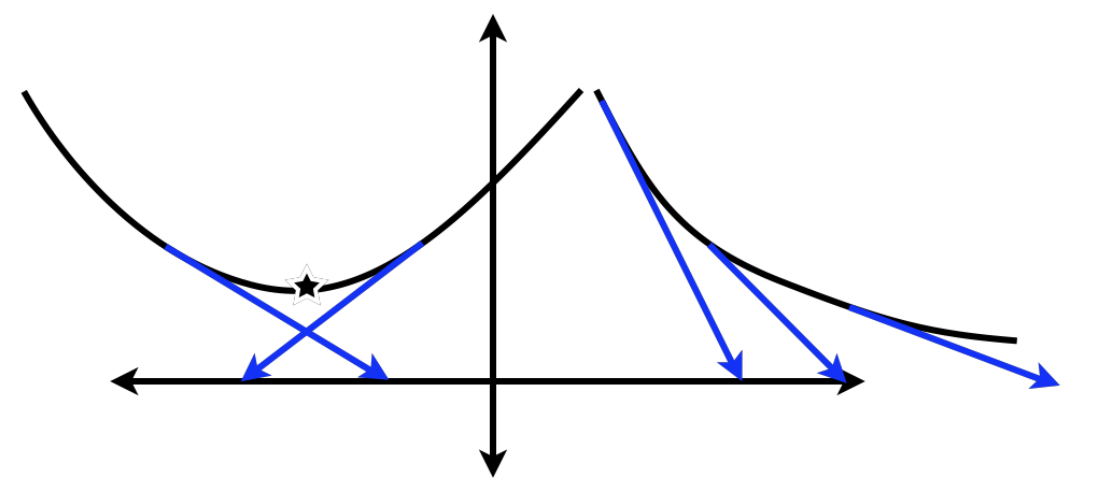
\includegraphics[width=0.98\linewidth]{figs/nle/failuremode1.png}
    \caption{Extrema/flat tails: Newton steps run away.}
    \end{subfigure}\hfill
    % ---- (b) cusp |x|^s ----
    \begin{subfigure}{0.48\linewidth}
    \centering
    % TODO: change to tikz
    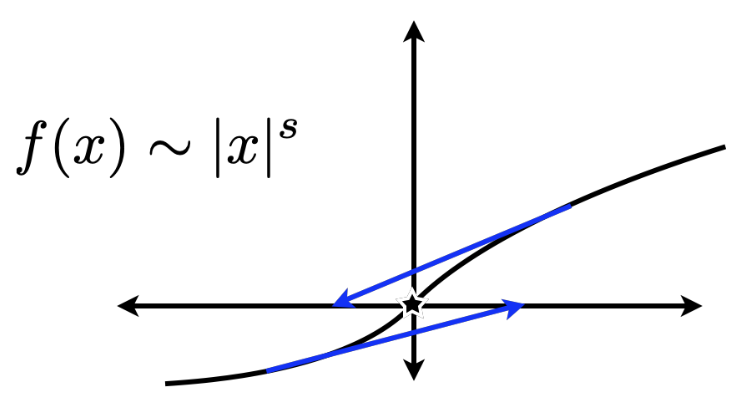
\includegraphics[width=0.98\linewidth]{figs/nle/failuremode2.png}
    \caption{Cusp $f(x)\approx|x|^{s}$: diverges $0<s<\frac12$; converges $\frac12<s<1$.}
    \end{subfigure}
    
    \caption{Newton's method failure modes (one Newton step shown in blue).}
    \label{fig:failure-modes}
\end{figure}
    
\subsubsection{Basins of Attraction:}
\label{par:basins-of-attraction}
Given a nonlinear system \(\vect{f}(\vect{x})=\vect{0}\), Newton's method updates
\[
\vect{x}_{k+1}=\vect{x}_k+\vect{d}_k,\qquad
\mat{J}(\vect{x}_k)\,\vect{d}_k=-\vect{f}(\vect{x}_k)
\]
where \(\mat{J}\) is the Jacobian. The \emph{basin of attraction} of a root \(\vect{x}^*\) is the set of initial guesses \(\vect{x}_0\) for which the iterates converge to \(\vect{x}^*\). When multiple roots exist, these basins can have complicated shapes; points near the boundaries of different basins often exhibit slow or erratic convergence because the local linearization (through \(\mat{J}\)) is nearly singular or unstable there.

\begin{exampleBox}
    \noindent\textbf{Example: Two Circles:}
    Consider the two-circle system
    \[
    \vect{f}(\vect{x})=
    \begin{bmatrix}
    (x_1+3)^2+(x_2+1)^2-9\\
    (x_1-2)^2+(x_2-2)^2-9
    \end{bmatrix}=\vect{0},
    \]
    which has two intersection points (two roots). The Jacobian is
    \[
    \mat{J}(\vect{x})=
    \begin{bmatrix}
    2(x_1+3) & 2(x_2+1)\\
    2(x_1-2) & 2(x_2-2)
    \end{bmatrix},
    \quad
    \det\mat{J}(\vect{x})
    =4\!\left[(x_1+3)(x_2-2)-(x_2+1)(x_1-2)\right]
    \]
    Expanding gives
    \[
    \det\mat{J}(\vect{x})=-12x_1+20x_2-16
    \quad\Longleftrightarrow\quad
    3x_1-5x_2+4=0
    \]
    This straight line is the \emph{singular set}: on it, the linear system for \(\vect{d}_k\) is singular, and near it the system is ill-conditioned. Consequently, initial guesses close to this line tend to require many Newton steps (or may fail unless a modification of Newton's method is used), whereas guesses well away from it converge rapidly to one of the two roots. The basin boundary between the two solutions usually tracks regions where \(\det\mat{J}\) changes sign or becomes small.

    \begin{center}
    \begin{tikzpicture}[scale=0.35]
    
        % ---------- plotting window ----------
        \draw[very thick] (-8,-8) rectangle (8,8);
        
        \begin{scope}
            % clip to the window
            \clip (-8,-8) rectangle (8,8);
          
            % tint ABOVE the line (upper LHS) light red
            \fill[red!20, fill opacity=.65]
                  (-8,8) -- (8,8) -- (8,5.6) -- (-8,-4) -- cycle;
          
            % tint BELOW the line (lower RHS) light blue
            \fill[cyan!20, fill opacity=.65]
                  (-8,-8) -- (8,-8) -- (8,5.6) -- (-8,-4) -- cycle;
          
            % the line on top
            \draw[line width=3pt, purple!70, opacity=.8, line cap=round]
                  (-8,-4) -- (8,5.6);
        \end{scope}
        
        % axes labels / corner ticks
        \node[below] at (0,-8) {$x_{1}$};
        \node[rotate=90] at (-8.5,0) {$x_{2}$};
        \node[below left]  at (-8,-8) {$-8$};
        \node[below right] at (8,-8) {$8$};
        \node[above left]  at (-8,8) {$-8$};
        \node[above right] at (8,8) {$8$};
        
        % ---------- circles ----------
        % C1: (x1-2)^2 + (x2-2)^2 = 9
        % C2: (x1+3)^2 + (x2+1)^2 = 9
        \path[name path=cOne] (2,2) circle (3);
        \path[name path=cTwo] (-3,-1) circle (3);
        
        \draw[very thick] (2,2) circle (3);
        \draw[very thick] (-3,-1) circle (3);
        
        % intersection stars
        \path [name intersections={of=cOne and cTwo, by={P,Q}}];
        \node[star, star points=5, star point ratio=2.1,
              draw=black, fill=white, inner sep=1.1pt] at (P) {};
        \node[star, star points=5, star point ratio=2.1,
              draw=black, fill=white, inner sep=1.1pt] at (Q) {};
        
        % small label for the red band (angle ~ arctan(0.6) ≈ 31°)
        \node[rotate=31, purple!70!black] at (1.8,2.4) {$\det \mathbf{J}(\vect{x})=0$};
        
    \end{tikzpicture}
    \end{center}
\end{exampleBox}

For some problems, the basin boundaries are not smooth curves but intricate fractals. A well-known example is solving \(f(z)=z^3-1=0\) in the complex plane. Newton's map
\begin{equation}
z_{k+1}=z_k-\frac{f(z_k)}{f'(z_k)}=z_k-\frac{z_k^3-1}{3z_k^2}=\frac{2z_k^3+1}{3z_k^2}
\end{equation}
has three attracting fixed points (the cube roots of unity). Each fixed point has its own basin of attraction, but the boundaries between these three basins are fractal and highly sensitive: tiny changes in the initial guess can send the iterates to a different root.

% TODO: add fractal basin boundary figure (if desired?)

\textbf{Practical note.} Near singular/ill-conditioned regions, methods such as damping/line search, trust-region steps, or continuation strategies can dramatically improve robustness, and plotting \(\det\mat{J}\) (or its condition number) alongside iteration counts is a helpful diagnostic when exploring basins of attraction.

\subsection{Approximating the Jacobian: Quasi-Newton Methods}
A significant computational cost in Newton's method comes from evaluating the Jacobian matrix and solving the associated linear system at each iteration. For complex systems, deriving an analytical expression for \(\mat{J}\) can be difficult and error-prone, and its evaluation can be expensive. This motivates quasi-Newton methods, which approximate \(\mat{J}\) or its inverse, often by low-rank updates built from secant information. The price typically paid is a reduction in the convergence rate from quadratic (for exact Newton under standard assumptions) to superlinear. Under poor conditions some schemes may be only linear, but under smoothness they often achieve superlinear behavior.

\subsubsection{1D Finite Differences} 
When an analytical derivative is unavailable, one can approximate it with finite differences. With step size \(\epsilon>0\), the first derivative satisfies
\begin{gather*}
  f'(x) \approx \frac{f(x+\epsilon)-f(x)}{\epsilon}
  \quad\text{(forward difference, truncation error }O(\epsilon)\text{),} \\
  f'(x) \approx \frac{f(x)-f(x-\epsilon)}{\epsilon}
  \quad\text{(backward difference, truncation error }O(\epsilon)\text{),} \\
  f'(x) \approx \frac{f(x+\epsilon)-f(x-\epsilon)}{2\epsilon}
  \quad\text{(centered difference, truncation error }O(\epsilon^2)\text{).}
\end{gather*}
The centered formula is often preferred for accuracy, though it generally requires two additional function evaluations at \(x\pm\epsilon\) even if \(f(x)\) is already known. These difference schemes are visualized below. 

\begin{center}
    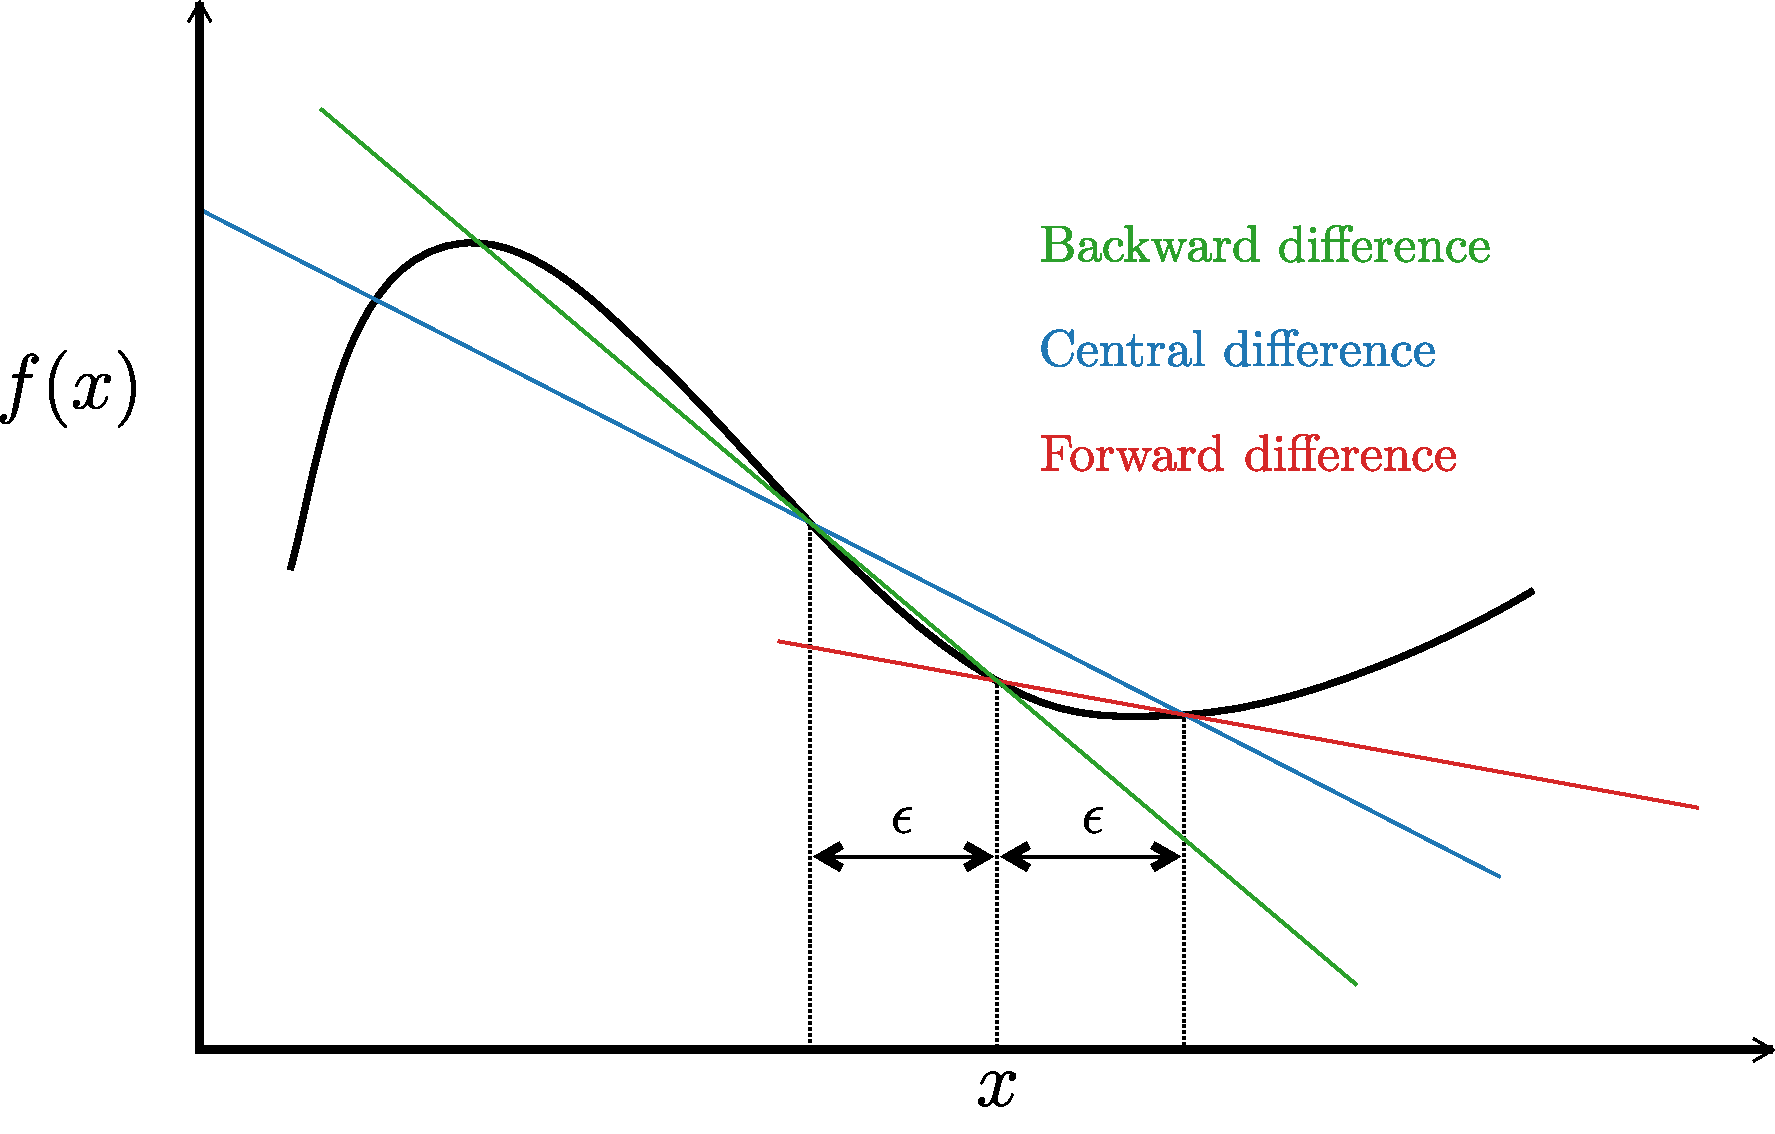
\includegraphics[width=.5\textwidth]{figs/nle/difference_schemes.pdf}
\end{center}

The choice of \(\epsilon\) is very important because two competing error sources balance against each other. If \(\epsilon\) is too large, the truncation error from neglecting higher-order terms dominates; for forward/backward differences this scales like \(O(\epsilon)\), while for the centered formula it scales like \(O(\epsilon^2)\). If \(\epsilon\) is too small, subtractive cancellation makes round-off error dominate when forming differences of nearly equal quantities; this round-off contribution is on the order of \(O(\epsilon_M/\epsilon)\) for these quotients, where \(\epsilon_M\) is the machine epsilon. Balancing these terms yields practical rules of thumb for the step size. For forward or backward differences one typically takes
\[
  \epsilon \approx \sqrt{\epsilon_M}\,\max\!\bigl(1,\lvert x\rvert\bigr)
\]
while for the centered difference a common choice is
\[
  \epsilon \approx \epsilon_M^{1/3}\,\max\!\bigl(1,\lvert x\rvert\bigr)
\]

\begin{exampleBox}
    \textbf{Example: Finite differences and the U-shaped error trade-off.}
    Consider estimating \(f'(1)\) for \(f(x)=e^x\) with the forward-difference quotient
    \[
      D_\epsilon f(1) = \frac{f(1+\epsilon)-f(1)}{\epsilon},
      \qquad \epsilon>0
    \]
    Two effects control the accuracy as \(\epsilon\) varies. The first is truncation error from the Taylor remainder (again, to be clear, we're using the Lagrange form of the remainder here):
    \[
      f(1+\epsilon) = f(1) + \epsilon f'(1) + \frac{1}{2}\epsilon^2 f''(\xi_\epsilon),
      \quad \text{so} \quad
      D_\epsilon f(1) - f'(1) = \frac{1}{2}\epsilon f''(\xi_\epsilon),
    \]
    which grows linearly like \(O(\epsilon)\). The second is round-off error from subtracting nearly equal numbers in floating-point arithmetic, which behaves like \(O(\epsilon_M/\epsilon)\). For \(f(x)=e^x\) at \(x=1\) we therefore expect the total error to behave like
    \[
      \underbrace{C_1\epsilon}_{\text{truncation}} + 
      \underbrace{C_2\frac{\epsilon_M}{\epsilon}}_{\text{round-off}}
      \quad \text{with} \quad C_1 \approx \frac{1}{2}e,\; C_2 \approx e,
    \]
    which produces a characteristic U-shaped curve when plotted against \(\epsilon\) on logarithmic axes. The minimum of this model occurs near
    \[
      \epsilon^\star \approx \sqrt{\frac{C_2}{C_1}\epsilon_M}
      \approx \sqrt{2\epsilon_M}
      \sim 10^{-8}
    \]
    in close agreement with the practical rule of thumb \(\epsilon \approx \sqrt{\epsilon_M}\,\max(1,|x|)\) for forward or backward differences. The figure below confirms this behavior numerically: as \(\epsilon\) decreases from coarse values, the error falls (truncation dominates), then rises again for very small \(\epsilon\) (round-off dominates).

    \begin{center}
        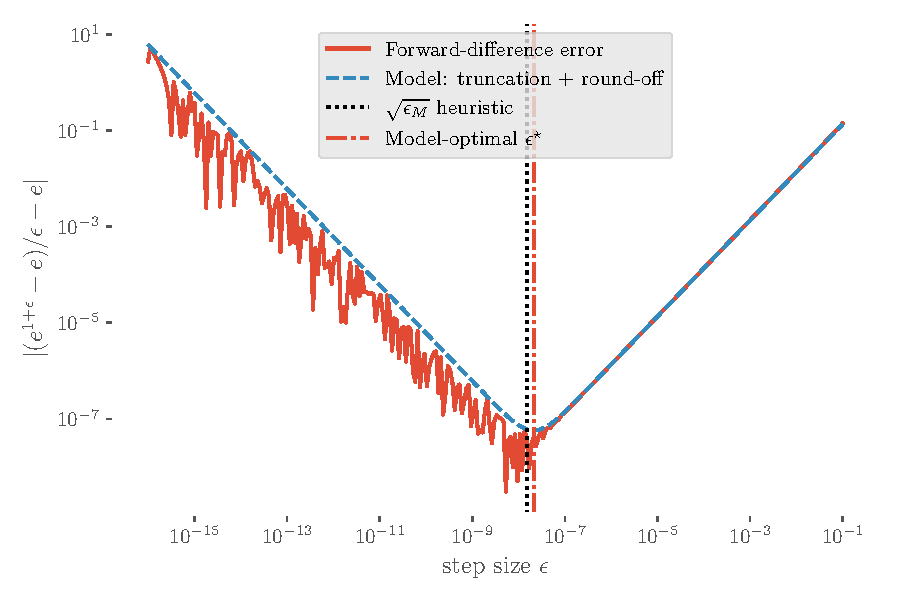
\includegraphics[width=.5\textwidth]{figs/nle/forward_difference_error.pdf}
    \end{center}
    
\end{exampleBox}


\subsubsection{ND Finite Differences (Approximating \texorpdfstring{$\mat{J}$}{J})}
For $\vect{f}:\mathbb{R}^n\!\to\!\mathbb{R}^n$ with components $f_i$, the Jacobian entries $J_{ij}(\vect{x})=\partial f_i/\partial x_j$ can be approximated by finite differences. A column-wise forward difference forms the $j$th column of $\mat{J}(\vect{x})$ by
\begin{equation}
  \mat{J}(\vect{x})\vect{e}_j
  \approx
  \frac{\vect{f}(\vect{x}+\epsilon_j \vect{e}_j)-\vect{f}(\vect{x})}{\epsilon_j},
  \qquad j=1,\ldots,n,
\end{equation}
where $\vect{e}_j$ is the $j$th standard basis vector and $\epsilon_j$ is a componentwise step. A scale-aware and numerically stable choice is
\begin{equation}
  \epsilon_j \approx \sqrt{\epsilon_M}\,\max\!\bigl(1,|x_j|\bigr),
\end{equation}
Constructing the full $n\times n$ Jacobian this way requires one evaluation of $\vect{f}(\vect{x})$ (usually already available from the current residual) and then one additional evaluation per column for a total of about $n$ extra function evaluations. Using centered differences improves accuracy but roughly doubles this columnwise cost to $2n$. When $\mat{J}$ is sparse, we can use techniques to group independent columns and cut the number of function evaluations substantially.

When we use a finite-difference Jacobian inside Newton's method, we expect linear or superlinear rates (it depends a bit on the details of the choice of Newton step).

\begin{exampleBox}
    \textbf{Example (MATLAB):} Below is an example MATLAB implementation of using column-wise forward differences to approximate the Jacobian:
    \begin{verbatim}
    function J = my_jacobian(x_current, Fhandle)
    % Column-wise forward-difference Jacobian with scale-aware steps.
    % x_current : n-by-1 vector
    % Fhandle   : function handle returning n-by-1 vector F(x)

        n = length(x_current);
        J = zeros(n, n);

        Fx = Fhandle(x_current);

        epsM   = eps;             % machine epsilon, defining for clarity
        h_base = sqrt(epsM);      % heuristic step magnitude

        for j = 1:n               % loop over columns
            x_pert = x_current;
            hj = h_base * max(1, abs(x_current(j)));
            if hj == 0
                hj = h_base;      % in case x_j is exactly zero
            end
            x_pert(j) = x_pert(j) + hj;

            F_pert = Fhandle(x_pert);
            J(:, j) = (F_pert - Fx) / hj;
        end
    end
    \end{verbatim}
\end{exampleBox}

\subsubsection{Broyden's Method (and other quasi-Newton updates)}
Rather than rebuilding a fresh finite-difference Jacobian at every iteration, we can instead update an approximation using secant information. Broyden's method maintains $\mat{B}_k \approx \mat{J}(\vect{x}_k)$ and enforces the latest secant equation with a minimal-rank correction:
\begin{equation}
  \mat{B}_{k+1}
  =
  \mat{B}_k
  +
  \frac{\bigl(\vect{y}_k - \mat{B}_k \vect{s}_k\bigr)\vect{s}_k^{\!T}}
       {\vect{s}_k^{\!T}\vect{s}_k},
  \qquad
  \vect{s}_k = \vect{x}_{k+1}-\vect{x}_k,
  \quad
  \vect{y}_k = \vect{f}(\vect{x}_{k+1})-\vect{f}(\vect{x}_k)
\end{equation}
At iteration $k$, we solve the linear system $\mat{B}_k \vect{d}_k = -\vect{f}(\vect{x}_k)$ and update $\vect{x}_{k+1}=\vect{x}_k+\vect{d}_k$. An initial $\mat{B}_0$ can be obtained from a finite-difference Jacobian, after which the rank-one updates avoid repeated full differencing. Under standard smoothness and regularity assumptions, these methods are typically superlinear, and in practice they can greatly reduce per-iteration cost while retaining robust local convergence behavior. We will revisit quasi-Newton methods in more detail in the optimization chapter.


\section{Continuation and Homotopy Methods}

Finding a good initial guess for Newton's method can be difficult, especially when a problem has multiple solutions. Where do starting points come from? And how can we be confident we've found \emph{all} the solutions?\footnote{``All solutions'' is generally unattainable without structure. For arbitrary nonlinear systems, it is impossible to decide or enumerate all solutions from finite samples alone.}  % TODO: Emphasize

This section introduces a powerful family of techniques for systematically exploring a problem's solution landscape. The core idea is simple: instead of solving one hard problem, we solve a sequence of related, easier ones. This general strategy is called continuation. A homotopy provides a general recipe for creating that sequence of problems. Together, they allow us to trace entire families of solutions as parameters change, generate excellent initial guesses for root-finders, and discover when new solutions appear or disappear at special points called bifurcations.

\subsection{Continuation}

Continuation turns a hard equation into a sequence of easy ones. Instead of attacking $f(x)=0$ head-on, we introduce a parameter $\lambda$ and consider a family $F(x,\lambda)=0$ so that:

\begin{enumerate}
\item the target problem appears at some $\lambda=\lambda_\star$, and
\item there is at least one value $\lambda=\lambda_0$ for which a solution is known or trivial.
\end{enumerate}

We then ``walk'' from $\lambda_0$ to $\lambda_\star$ in small steps, using the previously computed solution as the initial guess at the next step. The intuition here is simple: the solution we just found at the previous $\lambda$ value is an excellent initial guess for the next $\lambda$. You can plug that guess into any root finder you already know. If the solver struggles at some step, just reduce the $\lambda$ step size and try again.

% MC: can delete or comment this out, found it helpful when I was taking the course though
\textbf{Optional note.}\quad
We can show why small $\Delta\lambda$ $\Rightarrow$ small $\Delta x$ more formally (beyond just the intuition) by using the implicit function theorem. If $F(x_\star,\lambda_\star)=0$ and $\partial F/\partial x\neq 0$ at $(x_\star,\lambda_\star)$, the implicit function theorem gives a differentiable $x(\lambda)$ with $F(x(\lambda),\lambda)=0$ near $\lambda_\star$. Differentiating,
\begin{equation}
\frac{\partial F}{\partial x}\cdot x' + \frac{\partial F}{\partial \lambda} = 0 \implies x'(\lambda) = -\frac{\partial F/\partial \lambda}{\partial F/\partial x}.
\end{equation}
For a small step $\Delta\lambda$,
\begin{equation}
\Delta x := x(\lambda+\Delta\lambda)-x(\lambda)
= x'(\lambda)\,\Delta\lambda + O(\Delta\lambda^2)
= -\frac{\partial F/\partial \lambda}{\partial F/\partial x}\,\Delta\lambda + O(\Delta\lambda^2).
\end{equation}
Thus, $|\Delta x|$ is proportional to $|\Delta\lambda|$ as long as $\partial F/\partial x$ stays away from $0$, so the solution at $\lambda_k$ is an $O(\Delta\lambda)$-accurate initial guess for $\lambda_{k+1}$. We can derive a similar result for the multivariable case.

\textbf{Practical tips.}\quad You should choose $\Delta\lambda$ adaptively: increase it when Newton converges in a few iterations, and decrease it when convergence slows or fails. To discover multiple solution branches, start continuation from different initial seeds (from symmetry, asymptotics, or physical limits) and trace each branch to the target $\lambda_\star$. Also, as we will discuss in more detail later (and as suggested in the optional note above), it is important to monitor points where $\partial F/\partial x=0$ (or in general, points where the Jacobian is singular), as these can cause problems with parameter continuation.

Common uses include sweeping Reynolds or P\'eclet numbers in transport problems, temperature/pressure in phase equilibria, or rate constants in reaction networks.

\begin{exampleBox}
    \textbf{Example: Continuation for $f(x)=x^3-2x+1$.}
    
    Define the family
    $$
    f_{\lambda}(x)=x^3-2\lambda x+1,\qquad \lambda\in[0,1]
    $$
    so that $f_0(x)=x^3+1$ and $f_1(x)=f(x)$.
    
    At $\lambda=0$ there is an obvious root $x=-1$. We now sweep $\lambda$ from $0$ to $1$, carrying the last root forward as the next initial guess. In MATLAB-like pseudocode:
    
    \begin{verbatim}
    lambda = 0:0.01:1;
    xguess = -1;                  % solves f_0(x) = x^3 + 1 = 0
    
    for i = 1:length(lambda)
    f = @(x) x.^3 - 2*lambda(i).*x + 1;
    x(i) = fzero(@(x) f(x), xguess);   % any 1D solver works
    xguess = x(i);                     % continuation: carry forward
    end
    \end{verbatim}
    
    This produces a discrete approximation of the solution path $x(\lambda)$ and, in particular, a root for $\lambda=1$. If a step fails, reduce the increment in $\lambda$ near that region and try again. Below, we visualize the solution path.

    \begin{center}
        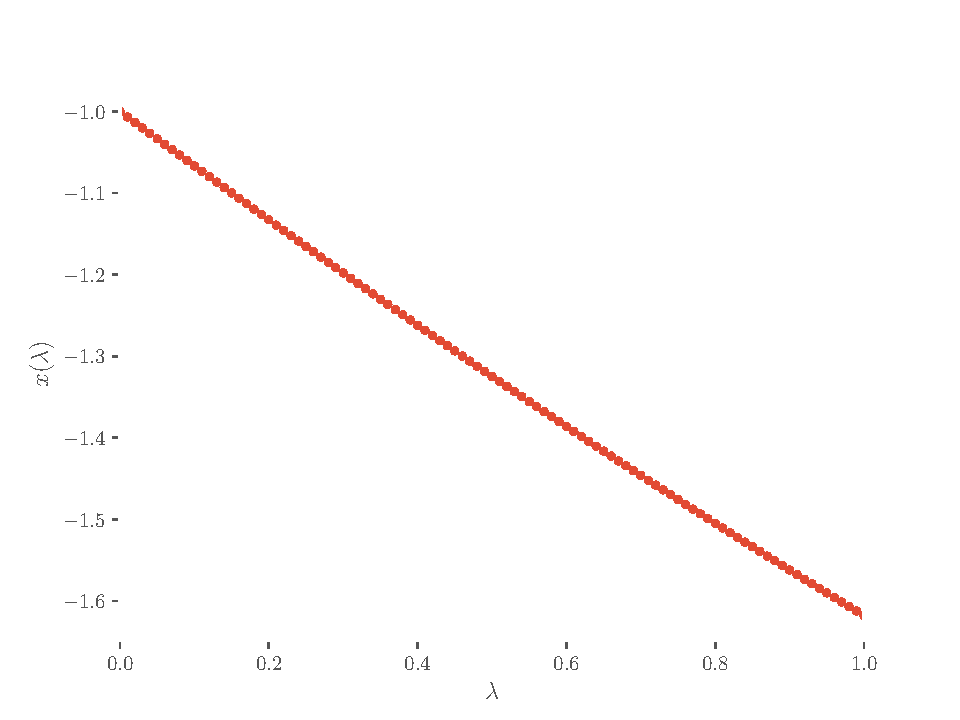
\includegraphics[width=.5\textwidth]{figs/nle/simple_continuation.pdf}
    \end{center}
    
    \emph{Optional extension (finding other roots).} The polynomial at $\lambda=1$ has three real roots. To trace other branches, rerun the same loop but start from a different seed. One practical trick is to start at a larger $\lambda$ (say $\lambda=10$) where the balances $x \approx 1/(2\lambda)$ or $x \approx \pm\sqrt{2\lambda}$ give three distinct initial guesses, then sweep $\lambda$ back down to $1$.
\end{exampleBox}

\subsection{Homotopy Methods}
Continuation works beautifully, but how do you choose the family of problems $F(x, \lambda)$? A \textbf{homotopy} provides a recipe for this. A homotopy continuously morphs a simple function into the target function. Given a hard system $\mathbf{f}(\mathbf{x}) = \mathbf{0}$, we pick a simple system $\mathbf{g}(\mathbf{x}) = \mathbf{0}$ that we know how to solve. We can then define the homotopy
\begin{equation}
    \mathbf{h}(\mathbf{x}, \lambda) = \lambda\,\mathbf{f}(\mathbf{x}) + (1-\lambda)\,\mathbf{g}(\mathbf{x}).
\end{equation}
which smoothly interpolates between the two systems if we start at \(\lambda=0\) and traverse to \(\lambda=1\).\footnote{By convention, we traverse from \(\lambda=0\) (the start system) to \(\lambda=1\) (the target), but in continuation and bifurcation analysis we treat \(\lambda\) as a free real parameter; allowing \(\lambda\notin[0,1]\) is often necessary to locate turning points and get around folds.
} At $\lambda=0$, we have the easy start system $\mathbf{g}(\mathbf{x}) = \mathbf{0}$, and at $\lambda=1$, we recover our target system $\mathbf{f}(\mathbf{x}) = \mathbf{0}$.

The obvious question is how to choose $\mathbf{g}(\mathbf{x})$. The only thing we really need is that $\mathbf{g}(\mathbf{x})$ has known roots, so the choice is very flexible. Some common ones include the following:
\begin{itemize}
    \item Fixed-point: $\mathbf{g}(\mathbf{x}) = \mathbf{x} - \mathbf{x}_0$, where $\mathbf{x}_0$ is a known starting point.
    \item Linear: $\mathbf{g}(\mathbf{x}) = \mathbf{A}\mathbf{x} - \mathbf{b}$, where you can easily solve the linear system for the starting roots.
\end{itemize}
But really, we can choose any $\mathbf{g}(\mathbf{x})$ that has known roots. Again, the key is that $\mathbf{g}(\mathbf{x})$ is easy to solve for the roots. In physical systems, we often have some simplified model that we know how to solve, and we can use that to construct the homotopy.
\begin{exampleBox}
    \textbf{Example: Fixed-point homotopy}
    We consider the target system
    \[
    \mathbf f(x,y)=
    \begin{bmatrix}
    x^2-1\\
    y^2-1
    \end{bmatrix}=\mathbf 0
    \]
    Obviously, we can analytically solve this simple system to find the roots, but we will use this as an example to illustrate the homotopy method. We choose a known point \((x_0,y_0)=(0.2,-0.5)\) and set
    \[
    \mathbf g(x,y)=
    \begin{bmatrix}
    x-x_0\\
    y-y_0
    \end{bmatrix}
    \]
    which allows us to define the homotopy
    \[
    \mathbf h(x,y,\lambda)
    =\lambda
    \begin{bmatrix}
    x^2-1\\ y^2-1
    \end{bmatrix}
    +(1-\lambda)
    \begin{bmatrix}
    x-x_0\\ y-y_0
    \end{bmatrix}
    =\mathbf 0,\qquad \lambda\in[0,1]
    \]
    At \(\lambda=0\), the unique root is clearly \((x,y)=(x_0,y_0)\). Because the coordinates decouple, for \(u\in\{x,y\}\) we solve a scalar quadratic at each \(\lambda\):
    \[
    \lambda(u^2-1)+(1-\lambda)(u-u_0)=0
    \implies
    \lambda u^2+(1-\lambda)u-\big[\lambda+(1-\lambda)u_0\big]=0.
    \]
    Following the root that satisfies \(u(0)=u_0\) traces a continuous path from \((x_0,y_0)\) to a solution of \(\mathbf f=\mathbf 0\).
    The figure shows the path in the \((x,y)\)-plane together with the lines \(x=\pm1\) and \(y=\pm1\).

    \begin{center}
        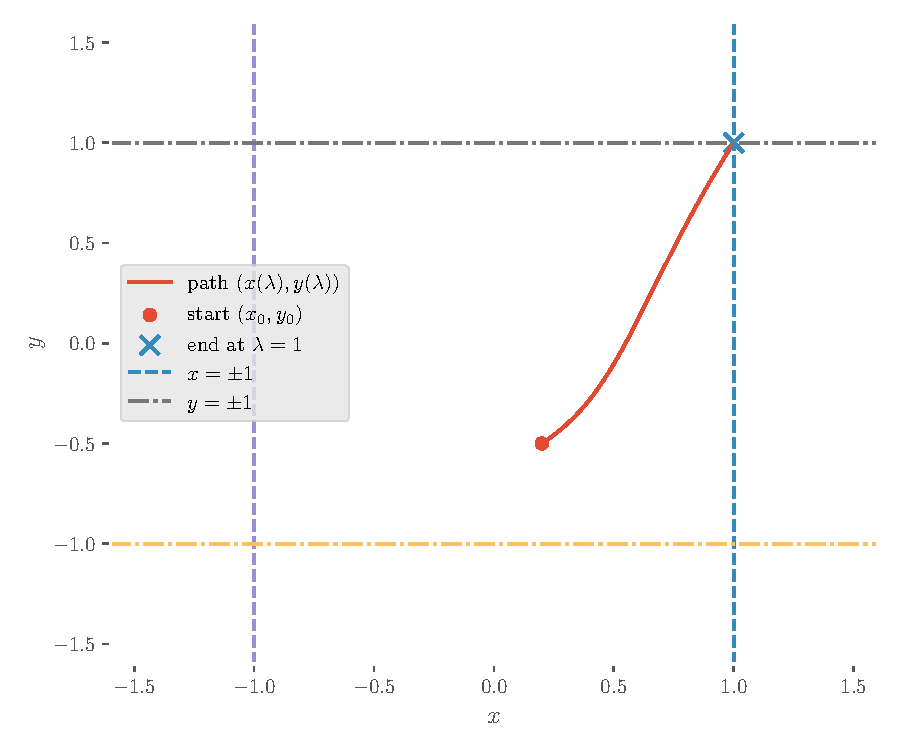
\includegraphics[width=0.7\textwidth]{figs/nle/fixed_point_path.pdf}
    \end{center}

\end{exampleBox}

\section{Bifurcation Analysis}
As the homotopy parameter $\lambda$ varies, the number of solutions of
\[
\mathbf{h}(\mathbf{x},\lambda)=\mathbf{0}
\]
can change. Sometimes this change happens discontinuously in the parameter: a solution branch folds back in $(\mathbf{x},\lambda)$-space so that, when viewed as a function of $\lambda$, a solution suddenly appears or disappears. Such events are called \textbf{turning points}. At a turning point, the Jacobian with respect to $\mathbf{x}$ becomes singular, and the usual implicit function theorem parameterization by $\lambda$ breaks down.

In other situations, additional solutions appear continuously: a previously single branch smoothly sprouts extra branches (for example, a symmetric branch splitting into three). These are called \textbf{bifurcations} (in the convention of 10.34). They are likewise characterized by a singular Jacobian: the rank of $\mathbf{J}_h=\partial \mathbf{h}/\partial \mathbf{x}$ drops and new directions of solutions open up.

In both cases, the event occurs at $(\mathbf{x}^*,\lambda^*)$ where $\mathbf{h}(\mathbf{x}^*,\lambda^*)=\mathbf{0}$ and the Jacobian is singular. So we can make the following definition:
\begin{definitionBox}
    \textbf{Definition: Bifurcation Point.}\quad A point $(\mathbf{x}^*,\lambda^*)$ is a bifurcation point of a homotopy $\mathbf{h}(\mathbf{x},\lambda)=\mathbf{0}$ if
    \begin{enumerate}
        \item $\mathbf{h}(\mathbf{x}^*,\lambda^*)=\mathbf{0}$ \quad (it lies on the solution set), and
        \item $\det \mathbf{J}_h(\mathbf{x}^*,\lambda^*)=0$ \quad (the Jacobian $\mathbf{J}_h=\partial \mathbf{h}/\partial \mathbf{x}$ is singular)
    \end{enumerate}
\end{definitionBox}
Near such points, solution branches either turn around in $\lambda$ (turning point) or split/merge continuously (bifurcation). Practically, we can detect them by monitoring the smallest singular value of $\mathbf{J}_h$ along a continuation, and we can locate them by solving an augmented system that enforces $\mathbf{h}=0$ together with singularity of $\mathbf{J}_h$:
\begin{equation}
    \begin{bmatrix}
    \mathbf{h}(\mathbf{x}^*,\lambda^*) \\
    \det \mathbf{J}_h(\mathbf{x}^*,\lambda^*)
    \end{bmatrix} = \mathbf{0}
\end{equation}
This is itself a nonlinear system that can be solved using Newton's method!

\begin{exampleBox}
    \textbf{Example: van der Waals equation via homotopy}
    Suppose we want to find the roots of the van der Waals equation of state for a given reduced pressure $\hat{P}$ and reduced temperature $\hat{T}$. The van der Waals equation is given in reduced form by
    \[
    f(\hat v)=\Bigl(\hat P+\frac{3}{\hat v^2}\Bigr)\Bigl(\hat v-\frac{1}{3}\Bigr)-\frac{8}{3}\hat T
    \]
    A clever idea here is to start from a simple model with a known solution (ideal gas), then continuously deform to the more realistic model (van der Waals) and track the root(s). For \(\hat P=0.1\), \(\hat T=0.5\), the ideal gas law has a known solution for these parameters:
    \[
    g(\hat v)=\hat P \hat v-\frac{8}{3}\hat T = 0
    \implies
    \hat v_0=\frac{8\hat T}{3\hat P}=\frac{4}{0.3} \approx 13.3
    \]
    Now, we can define the homotopy between these two systems as
    \[
    h(\hat v,\lambda)=\lambda f(\hat v)+(1-\lambda)g(\hat v),\qquad \lambda\in[0,1]
    \]
    At \(\lambda=0\), the root is the ideal-gas volume \(\hat v_0\). As \(\lambda\) increases, we track the solution(s) of \(h(\hat v,\lambda)=0\). A turning point for the homotopy is a pair $(\hat v^*,\lambda^*)$ with
    \[
    h(\hat v^*,\lambda^*)=0,
    \qquad
    \frac{\partial h}{\partial \hat v}(\hat v^*,\lambda^*)=0
    \iff
    \det \mathbf{J}_h(\hat v^*,\lambda^*)=0\ \text{(scalar case)}
    \]
    Substituting the derivative into the augmented system and then solving numerically produces two turning points and, correspondingly, the familiar S-shaped set of roots in $(\lambda,\hat v)$:
    \[
    (\lambda^*_1,\hat v^*_1)\approx(0.571,\,0.685),
    \qquad
    (\lambda^*_2,\hat v^*_2)\approx(1.692,\,6.764).
    \]
    Note that \(\lambda_2^*>1\). This is common with linear homotopies. Turning points can lie outside the interval \([0,1]\) even if we ultimately aim to reach \(\lambda=1\). For $\lambda<\lambda_1^*$ there is a single positive root. As $\lambda$ passes through $\lambda_1^*$, two additional roots appear and persist continuously up to $\lambda_2^*$, after which only one root remains. These points are highlighted in the figure below.
    \begin{center}
    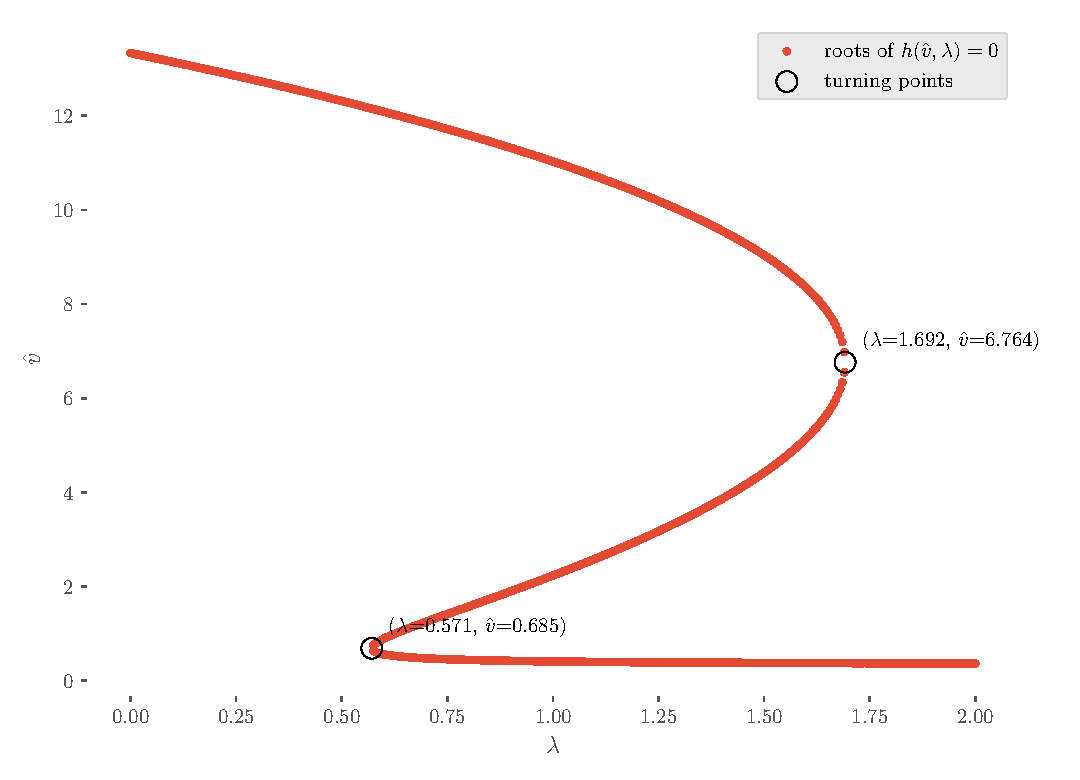
\includegraphics[width=0.80\linewidth]{figs/nle/vdw_homotopy_branches.pdf}
    \end{center}
\end{exampleBox}


% TODO: add circle example from lecture slides


\section{Damped Newton-Raphson}
% MC: I'm adding this context (not in the slides to make this less out of place -- still reads pretty weird though imo
When setting up the augmented system of equations to locate bifurcation points, the problem can be ill-scaled or sensitive, which can make vanilla Newton's method unreliable. A simple and effective safeguard is to damp the Newton step.

% MC: I think this part is pretty hand-wavy in its current form
To formalize this, let's refresh our memory on Newton's method. We wish to solve the nonlinear system 
\[
\mathbf{f}(\mathbf{x})=\mathbf{0}
\]
With vanilla Newton's method, the update rule is given by
\[
\mathbf{x}_{i+1}=\mathbf{x}_i-\mathbf{J}(\mathbf{x}_i)^{-1}\mathbf{f}(\mathbf{x}_i)
\]
Under this update rule, the iterates can behave erratically when we are far from a root. Newton's method is based on a linear (first-order) approximation that is only locally accurate in a small neighborhood. We make two important observations:
\begin{itemize}
  \item The \emph{direction} of the Newton step, 
  \(\mathbf{d}_i=-\mathbf{J}(\mathbf{x}_i)^{-1}\mathbf{f}(\mathbf{x}_i)\), is typically good: if we took a sufficiently small step in this direction, the residual norm 
  \(\lVert \mathbf{f}(\mathbf{x}_i+\alpha \mathbf{d}_i)\rVert_p\) 
  would decrease.
  \item The \emph{magnitude} of the step can be problematic: the size 
  \(\lVert \mathbf{d}_i\rVert_p=\lVert \mathbf{J}(\mathbf{x}_i)^{-1}\mathbf{f}(\mathbf{x}_i)\rVert_p\) 
  may be so large that the next iterate actually increases the residual (such that \( \lVert \mathbf{f}(\mathbf{x}_{i+1})\rVert_p \;>\; \lVert \mathbf{f}(\mathbf{x}_i)\rVert_p \)), which pushes us away from the solution instead of toward it.
\end{itemize}
Because our goal is to drive \(\lVert \mathbf{f}(\mathbf{x})\rVert_p \to 0\), we can correct this undesirable behavior by \emph{reducing the step size}. This leads to the damped Newton method:
\begin{definitionBox}
    \textbf{Definition: Damped Newton Method.}
    The damped Newton method is given by the update rule
    \begin{equation}
    \mathbf{x}_{i+1}=\mathbf{x}_i-\alpha\,\mathbf{J}(\mathbf{x}_i)^{-1}\mathbf{f}(\mathbf{x}_i),\qquad 0<\alpha\le 1
    \end{equation}
    Here, $\alpha$ is the damping parameter that controls the step size by reducing it.
\end{definitionBox}

\textbf{1D intuition and the ``right'' amount of damping.} In one dimension, the damped Newton method is
\begin{equation}
x_{i+1}=x_i-\alpha\,\frac{f(x_i)}{f'(x_i)}
\end{equation}
Ideally, we would pick the \(\alpha\) that minimizes the size of the residual after the step,
\begin{equation}
\alpha^\star = \argmin_{\alpha\in(0,1]}\; \left| f\!\left(x_i-\alpha\,\frac{f(x_i)}{f'(x_i)}\right) \right|
\end{equation}
With such a choice, we guarantee \(|f(x_{i+1})|<|f(x_i)|\) and avoid overshooting.

\begin{figure}[h]
    \centering
    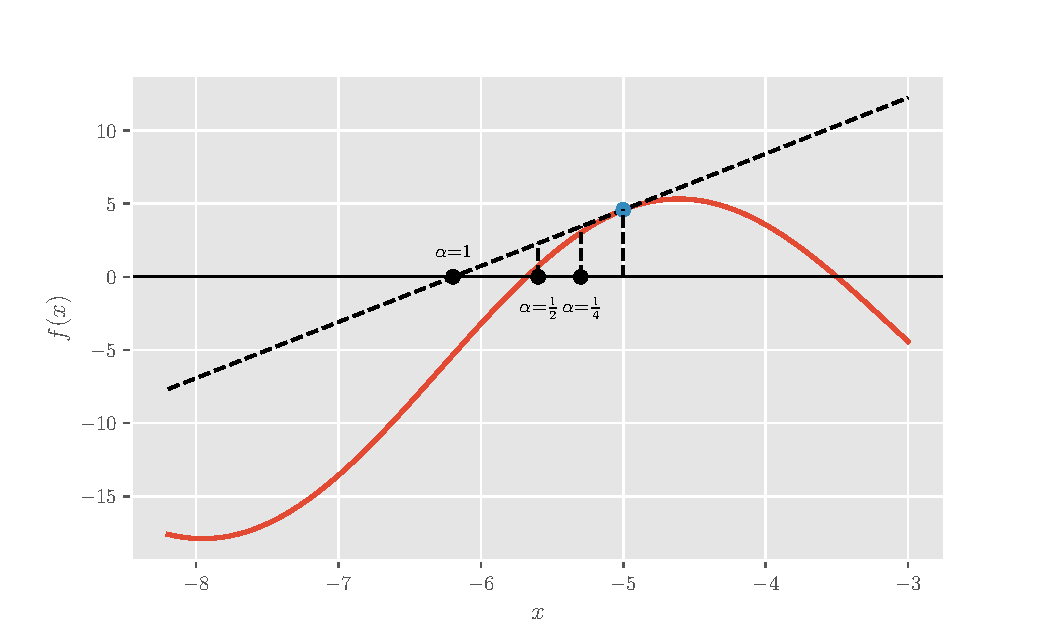
\includegraphics[width=0.7\textwidth]{figs/nle/damped_newton_verification.pdf}
    \caption{Damping in 1D prevents overshoot by shortening the Newton step along the same direction. We can see that here, $\alpha=1$ overshoots, while $\alpha=1/2$ and $\alpha=1/4$ do not.}
\end{figure}

\textbf{Many dimensions: line search on the Newton direction.}\quad In \(n\) dimensions, this generalizes to
\begin{equation}
\mathbf{x}_{i+1}=\mathbf{x}_i-\alpha\,\mathbf{J}(\mathbf{x}_i)^{-1}\mathbf{f}(\mathbf{x}_i),
\qquad
\alpha^\star=\arg\min_{0<\alpha\le 1}\;\bigl\|\mathbf{f}\bigl(\mathbf{x}_i-\alpha\,\mathbf{J}(\mathbf{x}_i)^{-1}\mathbf{f}(\mathbf{x}_i)\bigr)\bigr\|_p
\end{equation}
Computing \(\alpha^\star\) \emph{exactly} can be comparably hard and expensive as solving the original system, so we use an inexpensive \textbf{line search} that merely ensures the residual decreases. An example algorithm that implements this is shown below.

\begin{algorithm}[H]
\caption{Backtracking line search (damped Newton).}
\begin{enumerate}
\item Compute the Newton direction: \(\mathbf{d}_i=-\mathbf{J}(\mathbf{x}_i)^{-1}\mathbf{f}(\mathbf{x}_i)\).
\item Set \(\alpha\leftarrow 1\) (attempt the full Newton step).
\item While \(\;\lVert \mathbf{f}(\mathbf{x}_i+\alpha\mathbf{d}_i)\rVert_p \;>\; \lVert \mathbf{f}(\mathbf{x}_i)\rVert_p:\)
\begin{itemize}
  \item Set \(\alpha \leftarrow \alpha/2\) \hfill (backtrack)
\end{itemize}
\item Accept the step: \(\mathbf{x}_{i+1}=\mathbf{x}_i+\alpha\mathbf{d}_i\).
\end{enumerate}
\end{algorithm}

This strategy monotonically decreases \(\lVert \mathbf{f}\rVert_p\), which makes the method globally convergent: starting from any point, the sequence either converges to a root of \(\mathbf{f}\) or to a stationary point of the residual norm (a local minimum or a saddle point). We visualize this in \autoref{fig:damped_newton_2d_backtracking}.

\begin{figure}[h]
\centering
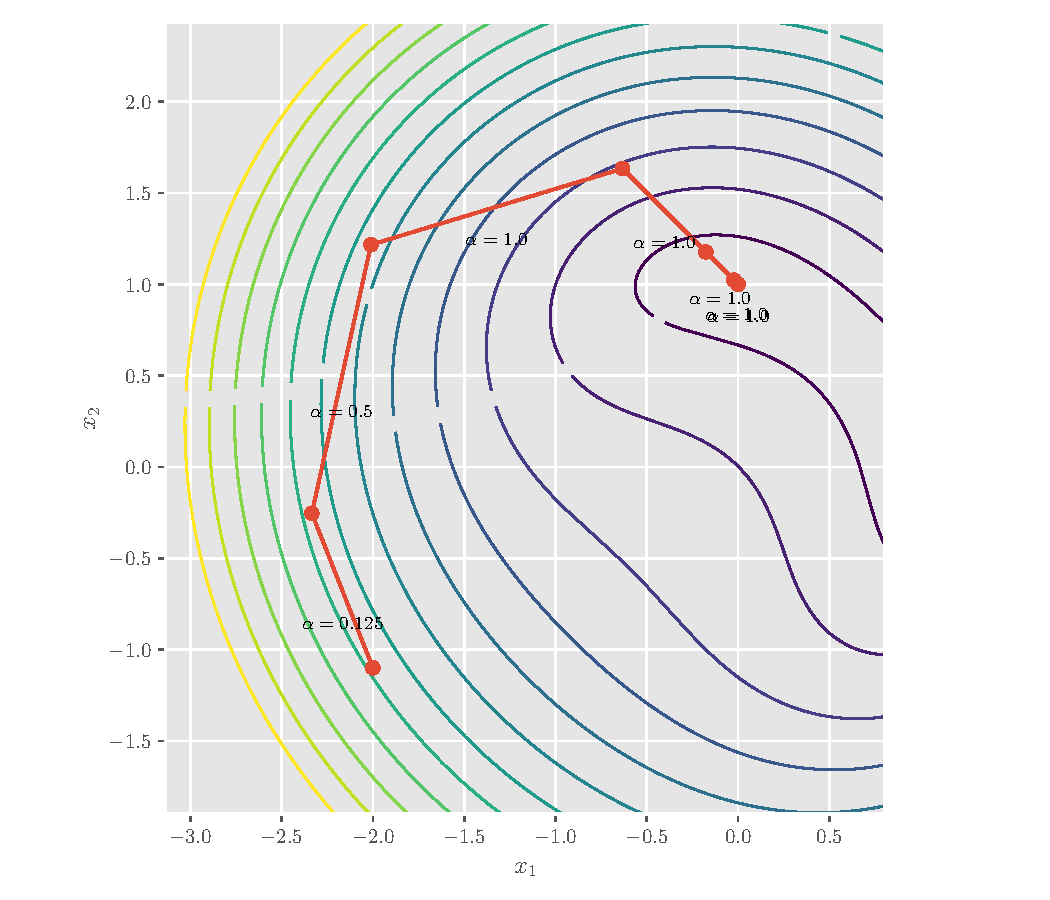
\includegraphics[width=0.7\textwidth]{figs/nle/damped_newton_2d_backtracking.pdf}
\caption{Backtracking line search for damped Newton on \(\mathbf{f}(x_1,x_2)=\big[x_1+x_2-1,\;x_1^2+x_2^2-1\big]\). Contours show level sets of \(\|\mathbf{f}(\mathbf{x})\|_2\), and dots trace the iterates from \(\mathbf{x}_0=(-2,-1.1)\). The full step (\(\alpha=1\)) is initially rejected; halving yields the first accepted step at \(\alpha=\tfrac{1}{8}\). Subsequent iterations accept \(\alpha=\tfrac12\) and then \(\alpha=1\) as the iterates approach a root, with the residual decreasing monotonically as guaranteed by the backtracking rule.}
\label{fig:damped_newton_2d_backtracking}
\end{figure}

% We can use any vector norm \(\lVert\cdot\rVert_p\) here, but the choice \(p=2\) is a common default due to its convergence properties. Additionally, the test above uses a simple decrease condition that
% \[
% \lVert \mathbf{f}(\mathbf{x}_i+\alpha\mathbf{d}_i)\rVert_p < \lVert \mathbf{f}(\mathbf{x}_i)\rVert_p
% \]
% but it is very common to replace it with a Armijo condition for stronger convergence guarantees. We'll see more about this in the optimization section.

\textbf{Convergence properties of damped Newton.}
Once the iterates enter a small neighborhood of a nonsingular root, the full Newton step ($\alpha=1$) is eventually accepted and quadratic convergence is recovered. With backtracking, the method is globally convergent to a stationary point of $\tfrac12\|f\|_2^2$ (if we use the 2-norm). Thus, it may converge to a root or to a nonroot stationary point (local minimum or saddle point) of the residual norm.

Looking ahead, other tweaks (trust regions, inexact Newton, etc.) can further improve reliability and are closely connected to optimization methods. We will revisit them in that context.

% MC: could be useful to have a summary here along with notes for practical considerations

%%% Local Variables:
%%% mode: LaTeX
%%% TeX-master: "../main"
%%% End:
